%%%%%%%%%%%%%%%%%%%%%%%%%%%%%%%%%%%%%%%%%
% Masters/Doctoral Thesis 
% LaTeX Template
% Version 2.5 (27/8/17)
%
% This template was downloaded from:
% http://www.LaTeXTemplates.com
%
% Version 2.x major modifications by:
% Vel (vel@latextemplates.com)
%
% This template is based on a template by:
% Steve Gunn (http://users.ecs.soton.ac.uk/srg/softwaretools/document/templates/)
% Sunil Patel (http://www.sunilpatel.co.uk/thesis-template/)
%
% Template license:
% CC BY-NC-SA 3.0 (http://creativecommons.org/licenses/by-nc-sa/3.0/)
%
%%%%%%%%%%%%%%%%%%%%%%%%%%%%%%%%%%%%%%%%%

%----------------------------------------------------------------------------------------
%	PACKAGES AND OTHER DOCUMENT CONFIGURATIONS
%----------------------------------------------------------------------------------------

\documentclass[
11pt, % The default document font size, options: 10pt, 11pt, 12pt
%oneside, % Two side (alternating margins) for binding by default, uncomment to switch to one side
english, % ngerman for German
singlespacing, % Single line spacing, alternatives: onehalfspacing or doublespacing
% draft, % Uncomment to enable draft mode (no pictures, no links, overfull hboxes indicated)
%nolistspacing, % If the document is onehalfspacing or doublespacing, uncomment this to set spacing in lists to single
%liststotoc, % Uncomment to add the list of figures/tables/etc to the table of contents
%toctotoc, % Uncomment to add the main table of contents to the table of contents
%parskip, % Uncomment to add space between paragraphs
%nohyperref, % Uncomment to not load the hyperref package
headsepline, % Uncomment to get a line under the header
%chapterinoneline, % Uncomment to place the chapter title next to the number on one line
%consistentlayout, % Uncomment to change the layout of the declaration, abstract and acknowledgements pages to match the default layout
openany
]{MastersDoctoralThesis} % The class file specifying the document structure

% \usepackage[utf8]{inputenc} % Required for inputting international characters
\usepackage[T1]{fontenc} % Output font encoding for international characters

\usepackage{mathpazo} % Use the Palatino font by default

% \usepackage[backend=bibtex,style=authoryear,natbib=true]{biblatex} % Use the bibtex backend with the authoryear citation style (which resembles APA)
\usepackage[backend=biber,style=authoryear,natbib=true]{biblatex} % Use the bibtex backend with the authoryear citation style (which resembles APA)

\addbibresource{references.bib} % The filename of the bibliography

\usepackage[autostyle=true]{csquotes} % Required to generate language-dependent quotes in the bibliography

%----------------------------------------------------------------------------------------
%	MARGIN SETTINGS
%----------------------------------------------------------------------------------------

\geometry{
	paper=a4paper, % Change to letterpaper for US letter
	inner=2.5cm, % Inner margin
	outer=3.8cm, % Outer margin
	bindingoffset=.5cm, % Binding offset
	top=1.5cm, % Top margin
	bottom=1.5cm, % Bottom margin
	%showframe, % Uncomment to show how the type block is set on the page
}

\setlength{\marginparwidth}{2.5cm}
\usepackage{caption}
\usepackage{subcaption}
\usepackage{hyperref}
\usepackage{enumitem}
\usepackage{booktabs}
\usepackage{amsmath}
\usepackage{cleveref}
\usepackage{xfrac}
\usepackage{multicol}
\usepackage{float}
\usepackage{cases}
\usepackage{pgfplots}
\usepackage{pgf-pie}
\usetikzlibrary{spy,arrows}
\graphicspath{ {images/} }

%----------------------------------------------------------------------------------------
%	THESIS INFORMATION
%----------------------------------------------------------------------------------------

\thesistitle{Corner localization and camera calibration from imaged lattices} % Your thesis title, this is used in the title and abstract, print it elsewhere with \ttitle
\supervisor{Dr. James \textsc{Pritts}} % Your supervisor's name, this is used in the title page, print it elsewhere with \supname
\examiner{} % Your examiner's name, this is not currently used anywhere in the template, print it elsewhere with \examname
\degree{Master of Science} % Your degree name, this is used in the title page and abstract, print it elsewhere with \degreename
\author{Andrii \textsc{Stadnik}} % Your name, this is used in the title page and abstract, print it elsewhere with \authorname
\addresses{} % Your address, this is not currently used anywhere in the template, print it elsewhere with \addressname

\subject{Data Science} % Your subject area, this is not currently used anywhere in the template, print it elsewhere with \subjectname
\keywords{} % Keywords for your thesis, this is not currently used anywhere in the template, print it elsewhere with \keywordnames
\university{\href{http://www.ucu.edu.ua}{Ukrainian Catholic University}} % Your university's name and URL, this is used in the title page and abstract, print it elsewhere with \univname
% \department{\href{http://department.university.com}{Faculty of Applied Sciences}} % Your department's name and URL, this is used in the title page and abstract, print it elsewhere with \deptname
% \group{\href{http://researchgroup.university.com}{Department of Computer Sciences}} % Your research group's name and URL, this is used in the title page, print it elsewhere with \groupname
% \faculty{\href{http://faculty.university.com}{}} % Your faculty's name and URL, this is used in the title page and abstract, print it elsewhere with \facname
\department{Faculty of Applied Sciences} % Your department's name and URL, this is used in the title page and abstract, print it elsewhere with \deptname
\group{Department of Computer Sciences} % Your research group's name and URL, this is used in the title page, print it elsewhere with \groupname
\faculty{} % Your faculty's name and URL, this is used in the title page and abstract, print it elsewhere with \facname

\AtBeginDocument{
\hypersetup{pdftitle=\ttitle} % Set the PDF's title to your title
\hypersetup{pdfauthor=\authorname} % Set the PDF's author to your name
\hypersetup{pdfkeywords=\keywordnames} % Set the PDF's keywords to your keywords
}

\begin{document}
\frontmatter % Use roman page numbering style (i, ii, iii, iv...) for the pre-content pages

\pagestyle{plain} % Default to the plain heading style until the thesis style is called for the body content

%----------------------------------------------------------------------------------------
%	TITLE PAGE
%----------------------------------------------------------------------------------------

\begin{titlepage}
	\begin{center}

		\vspace*{.06\textheight}
		{\scshape\LARGE \univname\par}\vspace{1.5cm} % University name
		\textsc{\Large Master Thesis}\\[0.5cm] % Thesis type

		\HRule \\[0.4cm] % Horizontal line
		{\huge \bfseries \ttitle\par}\vspace{0.4cm} % Thesis title
		\HRule \\[1.5cm] % Horizontal line

		\begin{minipage}[t]{0.4\textwidth}
			\begin{flushleft} \large
				\emph{Author:}\\
				% \href{http://www.johnsmith.com}{\authorname} % Author name - remove the \href bracket to remove the link
				\authorname % Author name - remove the \href bracket to remove the link
			\end{flushleft}
		\end{minipage}
		\begin{minipage}[t]{0.4\textwidth}
			\begin{flushright} \large
				\emph{Supervisor:} \\
				\href{https://prittjam.github.io/}{\supname} % Supervisor name - remove the \href bracket to remove the link  
			\end{flushright}
		\end{minipage}\\[3cm]

		\vfill

		\large \textit{A thesis submitted in fulfillment of the requirements\\ for the degree of \degreename}\\[0.3cm] % University requirement text
		\textit{in the}\\[0.4cm]
		\groupname\\\deptname\\[2cm] % Research group name and department name

		\vfill
		
\includegraphics[height=3cm]{UCU-Apps 2022.png} % University/department logo - uncomment to place it

		\vfill
		{\large Lviv 2022}\\[4cm] % Date

		\vfill
	\end{center}
\end{titlepage}

%----------------------------------------------------------------------------------------
%	DECLARATION PAGE
%----------------------------------------------------------------------------------------

\begin{declaration}
	\addchaptertocentry{\authorshipname} % Add the declaration to the table of contents
	\noindent I, \authorname, declare that this thesis titled, \enquote{\ttitle} and the work presented in it are my own. I confirm that:

	\begin{itemize}
		\item This work was done wholly or mainly while in candidature for a research degree at this University.
		\item Where any part of this thesis has previously been submitted for a degree or any other qualification at this University or any other institution, this has been clearly stated.
		\item Where I have consulted the published work of others, this is always clearly attributed.
		\item Where I have quoted from the work of others, the source is always given. With the exception of such quotations, this thesis is entirely my own work.
		\item I have acknowledged all main sources of help.
		\item Where the thesis is based on work done by myself jointly with others, I have made clear exactly what was done by others and what I have contributed myself.\\
	\end{itemize}

	\noindent Signed:\\
	\rule[0.5em]{25em}{0.5pt} % This prints a line for the signature

	\noindent Date:\\
	\rule[0.5em]{25em}{0.5pt} % This prints a line to write the date
\end{declaration}

\cleardoublepage

%----------------------------------------------------------------------------------------
%	QUOTATION PAGE
%----------------------------------------------------------------------------------------

% \vspace*{0.2\textheight}
%
% \noindent\enquote{\itshape Thanks to my solid academic training, today I can
% write hundreds of words on virtually any topic without possessing a shred of
% information, which is how I got a good job in journalism.}\bigbreak
%
% \hfill Dave Barry

%----------------------------------------------------------------------------------------
%	ABSTRACT PAGE
%----------------------------------------------------------------------------------------

\begin{abstract}
	\addchaptertocentry{\abstractname} % Add the abstract to the table of contents
	% The Thesis Abstract is written here (and usually kept to just this page). The page is kept centered vertically so can expand into the blank space above the title too\ldots

	Current state-of-the-art techniques occasionally fail to accurately estimate
	the camera parameters for wide-angle lenses, as most of the algorithms assume
	lenses with medium to small distortion. Partially it occurs due to extreme
	distortion at the edges of the image, which poses additional challenges to
	feature detection algorithms. We propose a novel approach for detecting
	additional features on the imaged calibration pattern using intermediate
	camera calibration. Utilizing the prior information about the calibration
	pattern's geometry, we can estimate the possible positions of the previously
	undetected features. Those features are filtered using the binary classifier,
	and the remaining ones are used to further constrain the camera calibration.
	The proposed method consists of three key steps: \((1)\) feature
	detection and estimation of the lattice geometry, \((2)\) initial camera
	calibration by solving the two-step linear minimization problem, and \((3)\)
	estimation of the possible positions of the undetected features by projecting the
	imputed and extended lattice geometry onto the image plane, and filtering them
	using the binary classifier.

  The code for this paper is available at
  \url{https://github.com/anstadnik/camera_calibration}.

	% In this paper, we propose a novel approach to camera calibration. We want to
	% use a robust solver to estimate the geometry between the correspondence of
	% points on the calibration pattern, which are called conjugate translations.
	% It is possible to use those
	% conjugate translations to predict the possible position of the previously
	% undetected calibration board features. We want to use the new points to constrain the camera calibration further. This process can be run iteratively,
	% refining the calibration board features, conjugate translations, and improving
	% the camera calibration.
\end{abstract}

%----------------------------------------------------------------------------------------
%	ACKNOWLEDGEMENTS
%----------------------------------------------------------------------------------------

\begin{acknowledgements}
	\addchaptertocentry{\acknowledgementname} % Add the acknowledgements to the table of contents
	I wish to thank the Armed Forces of Ukraine for protecting us. Thanks to those
	brave people I was able to study and work on this thesis. I want to thank my
	supervisor, Dr. James Pritts, for his guidance and support throughout the whole
	process of writing this thesis. I also want to express my gratitude to all of
	the people who encouraged me to keep going and inspired me to do my best: my
	groupmates, my friends, and my girlfriend.
	% The acknowledgments and the people to thank go here, don't forget to include your project advisor\ldots

	% \noindent If you was supported with the scholarship, please thank to your donor organization or a person who supported you.
\end{acknowledgements}

%----------------------------------------------------------------------------------------
%	LIST OF CONTENTS/FIGURES/TABLES PAGES
%----------------------------------------------------------------------------------------

\tableofcontents % Prints the main table of contents
%
% \listoffigures % Prints the list of figures
%
% \listoftables % Prints the list of tables

%----------------------------------------------------------------------------------------
%	ABBREVIATIONS
%----------------------------------------------------------------------------------------

% \begin{abbreviations}{ll} % Include a list of abbreviations (a table of two columns)
%
% 	\textbf{LAH} & \textbf{L}ist \textbf{A}bbreviations \textbf{H}ere\\
% 	\textbf{WSF} & \textbf{W}hat (it) \textbf{S}tands \textbf{F}or\\
%
% \end{abbreviations}

%----------------------------------------------------------------------------------------
%	PHYSICAL CONSTANTS/OTHER DEFINITIONS
%----------------------------------------------------------------------------------------

% \begin{constants}{lr@{${}={}$}l} % The list of physical constants is a three column table
%
% 	% The \SI{}{} command is provided by the siunitx package, see its documentation for instructions on how to use it
%
% 	Speed of Light & $c_{0}$ & \SI{2.99792458e8}{\meter\per\second} (exact)\\
% 	%Constant Name & $Symbol$ & $Constant Value$ with units\\
%
% \end{constants}

%----------------------------------------------------------------------------------------
%	SYMBOLS
%----------------------------------------------------------------------------------------

% \begin{symbols}{lll} % Include a list of Symbols (a three column table)
%
% 	$a$ & distance & \si{\meter} \\
% 	$P$ & power & \si{\watt} (\si{\joule\per\second}) \\
% 	%Symbol & Name & Unit \\
%
% 	\addlinespace % Gap to separate the Roman symbols from the Greek
%
% 	$\omega$ & angular frequency & \si{\radian} \\
%
% \end{symbols}

%----------------------------------------------------------------------------------------
%	DEDICATION
%----------------------------------------------------------------------------------------

% \dedicatory{For/Dedicated to/To my\ldots}

%----------------------------------------------------------------------------------------
%	THESIS CONTENT - CHAPTERS
%----------------------------------------------------------------------------------------

\mainmatter % Begin numeric (1,2,3...) page numbering

\pagestyle{thesis} % Return the page headers back to the "thesis" style

% Include the chapters of the thesis as separate files from the Chapters folder
% Uncomment the lines as you write the chapters

% \begin{enumerate}
	\item Introduction and motivation
	      \begin{enumerate}[label=(\alph*)]
		      \item Outline of the problem
		      \item Research objective
		            \begin{itemize}
			            \item Finding new features by projecting the board
			            \item Robustly classifying the true and false positives
		            \end{itemize}
		      \item Thesis structure
	      \end{enumerate}
	\item Related work
	      \begin{enumerate}[label=(\alph*)]
		      \item Camera calibration
		      \item Calibration boards
		      \item Feature detection on calibration boards
		      \item Camera models
		      \item Camera parameters estimation
		      \item Search of the previously undetected features
	      \end{enumerate}
	\item Background
	      \begin{enumerate}[label=(\alph*)]
		      \item Notation
		      \item Camera model
		            \begin{itemize}
			            \item Distortion model, inverse distortion model
			            \item Projection
			            \item Backprojection
		            \end{itemize}
		      \item Feature detection
		      \item Camera calibration (Probably I could move it to the Approach)
	      \end{enumerate}
	\item Approach
	      \begin{enumerate}[label=(\alph*)]
		      \item Feature detection
		      \item Camera calibration
		      \item Board projection, features classification
	      \end{enumerate}
	\item Experiments \todo{I'll have to merge something to have 5 chapters}
	      \begin{enumerate}[label=(\alph*)]
		      \item Synthesizer
		      \item Datasets
		      \item Metrics
		      \item Results
	      \end{enumerate}
	\item Conclusions
\end{enumerate}




\chapter{Introduction and motivation}\label{cha:introduction_and_motivation}

\section{Outline of the problem}\label{sec:outline_of_the_problem}

Better camera calibration improves the performance of various downstream tasks
by providing a more accurate mapping between 3D world coordinates and 2D image
plane coordinates. This improved mapping enables precise alignment, positioning,
and scaling of objects within the scene. By determining the camera's intrinsic
and extrinsic parameters, algorithms can correct for lens distortion, estimate
depth information, and accurately overlay virtual content. Consequently, tasks
such as 3D reconstruction, augmented reality, and object detection can achieve
better results in terms of precision, spatial consistency, and overall visual
quality.

Although manufacturers can estimate camera calibration parameters a priori,
fully automatic calibration is often preferred, especially when camera metadata
is unavailable. Currently, wide-angle lenses, particularly in mobile phones and
GoPro-type cameras, dominate consumer photography. These cameras pose additional
challenges due to their requirement for highly non-linear models with numerous
parameters. The high distortion of the image plane also makes finding key points
robustly challenging.

Typically, camera calibration is obtained by capturing an image of a known
calibration pattern, which is then used to estimate the camera parameters.
Alternatively, some methods do not use a calibration pattern but instead infer
geometric constraints directly from the scene. However, this approach is
generally less accurate.

As reported by \textcite{duisterhofTartanCalibIterativeWideAngle2022} on
\citedate{duisterhofTartanCalibIterativeWideAngle2022}, the current state-of-the-art
methods
\cite{olsonAprilTagRobustFlexible2011}
\cite{schopsWhyHaving102020} \cite{krogiusFlexibleLayoutsFiducial2019}
fail on images with high distortion.
\textcite{duisterhofTartanCalibIterativeWideAngle2022} suggested an iterative
the approach of image undistortion and target reprojection, achieving the superior
robustness to the noise than the state-of-the-art methods because the feature
detection is performed on the undistorted image.

Instead of searching for the features on the undistorted image, it is possible to
use conjugate translations \cite{schaffalitzkyGeometricGroupingRepeated1998},
to predict the position of the previously undetected feature points and to
further, constrain the camera calibration.
\textcite{prittsMinimalSolversRectifying2021} showed that three pairs of points,
related by the same translations on the scene plane are sufficient to estimate
the camera calibration and the parameters of the conjugate translations.

We want to use the work of \textcite{prittsMinimalSolversRectifying2021} to bootstrap
the camera calibration, and then use the found conjugate translations and camera
parameters to iteratively predict and refine the positions of the calibration
board features, calibration parameters, and conjugate translations.

\section{Thesis structure}\label{sec:thesis_structure}

This paper has the following structure: in \autoref{sec:related_work}, we will describe the related work, including the
literature search method and methodology, various subtopics of the camera
calibration, mention conjugate translations, and outline the state-of-the-art
solutions. We define the research gap in \autoref{sec:gap_analysis} and outline
the proposed approach to solution and evaluation in
\autoref{sec:problem_setting_and_approach_to_solution}. We will describe the
early results in \autoref{sec:early_results_and_discussion}, including the
dataset analysis, feature detector, and conjugately translated points simulator.
In \autoref{sec:summary_and_future_work}, we will summarize the results and
outline future work.
\todo{Update}

\endinput

\chapter{Related work}\label{cha:related_work}

\section{Camera calibration}\label{sub:camera_calibration}

Getting the correspondence between the spatial
and the image coordinates requires camera calibration. Camera
calibration consists of the geometric camera model and the parameters of this
model. That information makes it possible to obtain the 2d image coordinates
of any point in the 3d space.

Usually, the geometric camera model is obtained from the domain knowledge of the
researcher or the camera manufacturer. Often, they choose the simplified model as
a trade-off between accuracy and complexity. The model's parameters are usually
obtained by solving the constrained optimization problem, given the set of
points with known geometry.

\section{Calibration boards}\label{sub:calibration_boards}

To achieve a robust calibration, images with repeating patterns are
usually used. The camera
calibration parameters can be found using prior knowledge of the properties of
the pattern, such that the pattern invariants hold on
the image. Initially, the chessboard~\citep{OpenCVCameraCalibration,
v.douskosAutomaticCalibrationDigital2007} patterns were used
(\cref{fig:chessboard}).

Later, ArUco
~\citep{garrido-juradoAutomaticGenerationDetection2014} (\cref{fig:gboriginal}) and
AprilTag~\citep{olsonAprilTagRobustFlexible2011a} (\cref{fig:apriltag})
allowed detecting the
orientation of the pattern, as well as uniquely identifying each located pattern
even under occlusion. Based on ArUco,
ChArUcO~\citep{OpenCVCameraCalibration} (\cref{fig:charuco}) was
proposed as more robust.

\begin{figure}[h]
	\centering
	\begin{subfigure}[b]{0.45\textwidth}
		\centering
		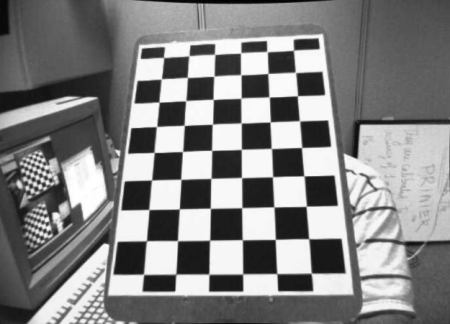
\includegraphics[width=\linewidth]{chessboard.png}
		\caption{Chessboard~\cite{OpenCVCameraCalibration}}
		\label{fig:chessboard}
	\end{subfigure}
	\hfill
	\begin{subfigure}[b]{0.45\textwidth}
		\centering
		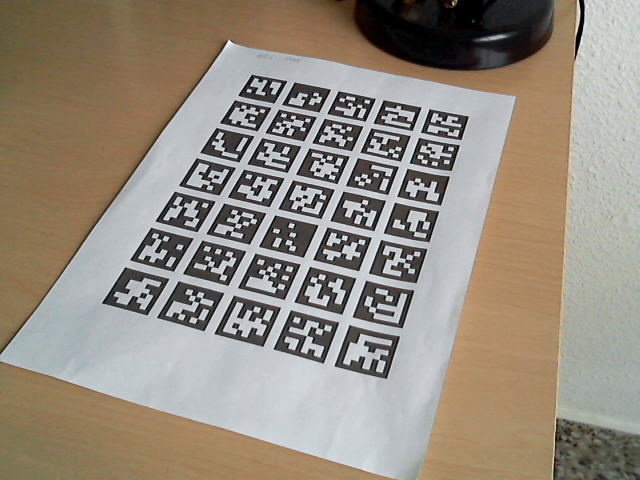
\includegraphics[width=\linewidth]{gboriginal.png}
		\caption{ArUco board~\cite{OpenCVDetectionArUco}}
		\label{fig:gboriginal}
	\end{subfigure}
	\begin{subfigure}[b]{0.45\textwidth}
		\centering
		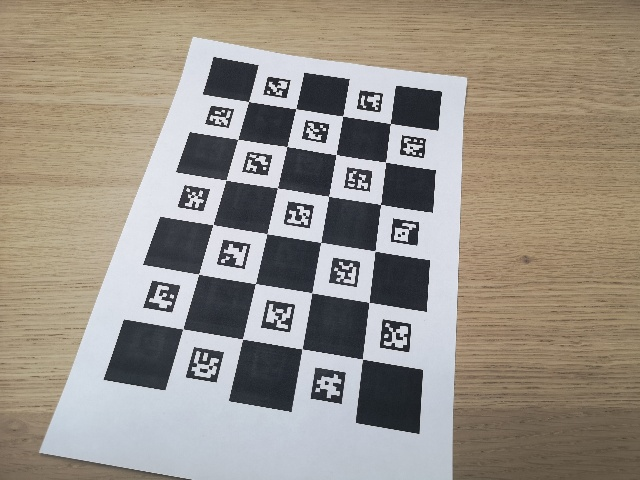
\includegraphics[width=\linewidth]{charuco.png}
		\caption{Charuco board~\cite{OpenCVDetectionChArUco}}
		\label{fig:charuco}
	\end{subfigure}
	\hfill
	\begin{subfigure}[b]{0.45\textwidth}
		\centering
		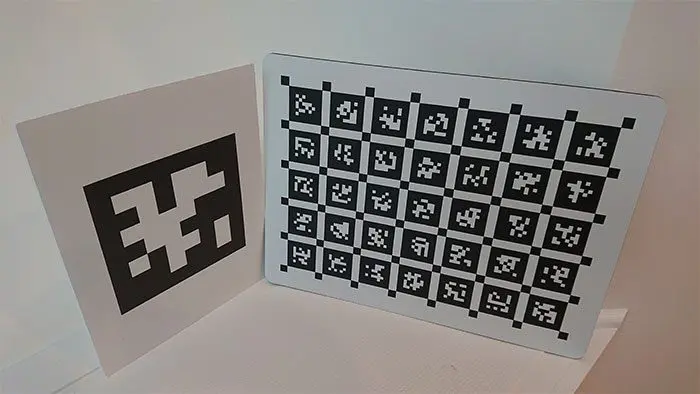
\includegraphics[width=\linewidth]{apriltag.png}
		\caption{AprilTag board~\cite{rosebrockAprilTagPython2020} (right)}
		\label{fig:apriltag}
	\end{subfigure}
	\caption{Calibration boards.}
\end{figure}

\section{Camera models}\label{sub:camera_models}

The choice of the camera model depends on the camera's physical properties
and the accuracy required. Usually, the parametric models are simpler to use, as
they have only a few parameters and deliver good accuracy.
The most common are the Double Sphere
model~\citep{usenkoDoubleSphereCamera2018}, the Kannala-Brandt
model~\citep{kannalaGenericCameraModel2006}, and the Field-of-View
model~\citep{devernayStraightLinesHave2001}.
In the ill-posed problem of camera calibration, the common choice
of the camera model is the division
model~\citep{fitzgibbonSimultaneousLinearEstimation2001}.
However, \cite{schopsWhyHaving102020} shows that they tend to have
significantly higher errors than the non-parametric (general) models.
The \cite{lochmanBabelCalibUniversalApproach2021} suggested a framework for
converting the parameters of a powerful back-projection
\cite{zhangFlexibleNewTechnique2000} model to recover different models' parameters.

\section{Camera parameters estimation}\label{sub:camera_parameters_estimation}

Camera calibration using repeating patterns was an important subject for a long
time, for example, \cite{schaffalitzkyGeometricGroupingRepeated1998} in
\citeyear{schaffalitzkyGeometricGroupingRepeated1998} and
\cite{zhangFlexibleNewTechnique2000}.

% Camera calibration is a crucial step for many computer vision tasks,
% hence many methods were proposed to solve this problem (e.g.,
% ~\cite{brownCloseRangeCameraCalibration1971},
% ~\cite{heikkilaFourstepCameraCalibration1997},
% ~\cite{fitzgibbonSimultaneousLinearEstimation2001},
% ~\cite{sturmGenericConceptCamera2004},
% ~\cite{clausRationalFunctionLens2005},
% ~\cite{meiSingleViewPoint2007},
% ~\cite{ramalingamUnifyingModelCamera2017}).

Nevertheless, camera calibration is still an open problem; recently,
multiple new approaches have arisen.
\cite{lochmanBabelCalibUniversalApproach2021} suggest a universal approach
to camera calibration, with a separate step of converting between camera models.
\cite{huDeepChArUcoDark2019} used deep learning to detect ChArUcO boards.
Recently, on \citedate{duisterhofTartanCalibIterativeWideAngle2022},
\cite{duisterhofTartanCalibIterativeWideAngle2022} introduced the iterative
approach to camera calibration, which outperforms the previous state-of-the-art
approaches for wide-angle cameras.

\todo{Add the paper about the feature detection}

% The camera calibration depends a lot on the physical camera properties, choice
% of the camera model, calibration method, number of images used for calibration,
% prior knowledge of the camera, and many other variables. Therefore, currently,
% there is no established method of general camera calibration approach
% comparison, and the state-of-the-art is not well-defined. However, it is possible
% to compare the methods in the context of specific tasks and datasets.


\chapter{Background}\label{cha:background}



\chapter{Approach}\label{cha:approach}

\section{Feature detection}\label{sec:feature_detection}

For the feature detection, we used the approach proposed by
\cite{geigerAutomaticCameraRange2012} (see \cref{sec:boards_features_detection,
	feature_detection}).
\missingfigure{Show the feature detection results.}

\section{Camera calibration}\label{sec:camera_calibration}

In this work, we obtained the camera calibration in two steps: first, we
used the approach, proposed by \cite{scaramuzzaToolboxEasilyCalibrating2006} to
obtain the initial approximation of the camera parameters. Then, we used the
optimization to minimize the reprojection error between the board and the
back-projected corners.

\subsection{Reprojection error}\label{sub:reprojection_error}

The reprojection error is the distance between the reprojected point and the
measured one. It is used to evaluate the quality of the camera calibration.

We chose to minimize the reprojection error between the board and back-projected
corners, which were initially detected. The projection and back-projection are
the inverse of each other, hence minimizing the error between the projection of
the board and the detected corners and minimizing the error between the
back-projection of the detected corners and the board are
equivalent\todo{Doesn't sound very rigorous to me.}. We minimized the error
between the board and the back-projected corners because back-projection does
not require the root finding.

Let's define the following variables: \(\boldsymbol{\theta} = \begin{pmatrix}
	\theta_x, \theta_y, \theta_z
\end{pmatrix}^{T}\) is the vector of Euler rotation angles, \(\mathbf{t} = \begin{pmatrix}
	t_x, t_y, t_z
\end{pmatrix}^{T}\) is the translation vector, \(\boldsymbol{\lambda} = \begin{pmatrix}
	\lambda_1, \lambda_2
\end{pmatrix}^{T}\)\todo{Justify why we used 2} is the intrinsic parameters vector, \(\) is the focal
length, and \(\mathbf{s} = \begin{pmatrix}
	s_x, s_y
\end{pmatrix}^{T}\) is the sensor size\todo{Make sure I'm using the correct terms.}.
From the input image, we know the resolution \(\mathbf{r} = \begin{pmatrix}
	r_x, r_y
\end{pmatrix}^{T}\).
From the rotation vector, we can compute the rotation matrix \(\mathbf{R}\) as:

From \(\boldsymbol{\theta}\), the rotation matrix $R$ can be calculated as follows:

\begin{equation}
	R = R(\theta_x) R(\theta_y) R(\theta_z)
\end{equation} \todo{Is the notation ok?}

where

\begin{align}
	% R_x(\phi)   & =
	% \begin{bmatrix}
	% 	1 & 0          & 0           \\
	% 	0 & \cos(\phi) & -\sin(\phi) \\
	% 	0 & \sin(\phi) & \cos(\phi)
	% \end{bmatrix} \\
	% R_y(\theta) & =
	% \begin{bmatrix}
	% 	\cos(\theta)  & 0 & \sin(\theta) \\
	% 	0             & 1 & 0            \\
	% 	-\sin(\theta) & 0 & \cos(\theta)
	% \end{bmatrix}                 \\
	% R_z(\psi)   & =
	% \begin{bmatrix}
	% 	\cos(\psi) & -\sin(\psi) & 0 \\
	% 	\sin(\psi) & \cos(\psi)  & 0 \\
	% 	0          & 0           & 1
	% \end{bmatrix}
	R(\theta_x) & =
	\begin{bmatrix}
		1 & 0              & 0               \\
		0 & \cos(\theta_x) & -\sin(\theta_x) \\
		0 & \sin(\theta_x) & \cos(\theta_x)
	\end{bmatrix} \\
	R(\theta_y) & =
	\begin{bmatrix}
		\cos(\theta_y)  & 0 & \sin(\theta_y) \\
		0               & 1 & 0              \\
		-\sin(\theta_y) & 0 & \cos(\theta_y)
	\end{bmatrix} \\
	R(\theta_z) & =
	\begin{bmatrix}
		\cos(\theta_z) & -\sin(\theta_z) & 0 \\
		\sin(\theta_z) & \cos(\theta_z)  & 0 \\
		0              & 0               & 1
	\end{bmatrix}
\end{align}

Then, \(H\) is given by:
\begin{equation}
	H = \begin{bmatrix}
		\mathbf{r_1} & \mathbf{r_2} & \mathbf{t}
	\end{bmatrix}.
\end{equation}

We can compute the intrinsic camera matrices as follows:
\begin{equation}
	K = \begin{pmatrix}
		\frac{f r_x}{s_x} & 0                 & \frac{r_x}{2} \\
		0                 & \frac{f r_y}{s_y} & \frac{r_y}{2} \\
		0                 & 0                 & 1
	\end{pmatrix},
\end{equation}.

Then, the back-projection of a 2D point \(\mathbf{u} = \begin{pmatrix}
	u, v, 1
\end{pmatrix}\) into a scene point with \(Z = 0\) \(\mathbf{X} = \begin{pmatrix}
	X, Y, 1
\end{pmatrix}\) is given by:
\begin{equation}
	\mathbf{X} = H g_{\lambda_1, \lambda_2}(K^{-1} \mathbf{u}).
\end{equation}

\subsection{Initial approximation}\label{sub:initial_approximation}

\cite{scaramuzzaToolboxEasilyCalibrating2006} proposed an automatic method for
camera calibration, which consisted of the following steps:
\begin{itemize}
	\item Solving for the camera extrinsic parameters
	\item Solving for the camera intrinsic parameters
	\item Linear refinement of the intrinsic and extrinsic parameters
	\item Iterative center detection
	\item Non-linear refinement
\end{itemize}

In this work, we focused on the single image, while the original approach relied
on the multiple images. Therefore, we used only the first two steps of the
algorithm.

\subsubsection{Solving for the camera extrinsic parameters}\label{ssub:solving_for_the_camera_extrinsic_parameters}

To derive the solver for the camera extrinsic parameters, start from
\cref{eq:projection}:
\begin{align}
	\alpha \mathbf{u}                                  & = K f(H\mathbf{X})                  \\
	\alpha K^{-1} \mathbf{u}                           & = f(H\mathbf{X})    &  &
	\text{Move \(K\) to the left side}                                                       \\
	\alpha g( K^{-1}\mathbf{u})                        & = g(f(H\mathbf{X})) &  &
	\text{Set \(\mathbf{\widehat{u}} = K^{-1}\mathbf{u}\); apply \(g(\cdot)\) to both sides} \\
	\alpha \begin{pmatrix}
		       \widehat{u}_x \\ \widehat{u}_y \\ \psi(r(\mathbf{\widehat{u}}))
	       \end{pmatrix}^{T} & = H\mathbf{X}                                 \\
\end{align}

For \(K\) we used the placeholder values. \(f\) was set to a constant value for
the typical consumer camera, and \(c_x, c_y\) were set to the center of the
image.
The correct values will be computed during the optimization \cref{sub:optimization}.

To eliminate the dependency on the scale \(\alpha\), multiply both sides
vectorially by \(g(\mathbf{\widehat{u}})\):
\begin{equation}
	\alpha g(\mathbf{\widehat{u}}) \times g(\mathbf{\widehat{u}})
	= g(\mathbf{\widehat{u}}) \times H\mathbf{X}
	= 0 \implies
	\begin{pmatrix}
		\widehat{u}, \widehat{v}, \psi(r(\mathbf{\widehat{u}}))
	\end{pmatrix}^{T} \times \begin{bmatrix}
		\mathbf{r_1} & \mathbf{r_2} & \mathbf{t}
	\end{bmatrix}^{T} \mathbf{X} = 0
	\label{eq:eq_no_multiplier}
\end{equation}.

From \cref{eq:eq_no_multiplier}, we can see that a point contributes to three
homogeneous equations:
\begin{align}
	\widehat{v} (t_1X + t_2 Y + t_3) -
	g(r(\mathbf{\widehat{u}})) (r_{12}X + r_{22}Y + t_2 ) & = 0
	\label{eq:scaramuzza_system_1}                              \\
	g(r(\mathbf{\widehat{u}})) (r_{11}X + r_{12}Y + t_1) -
	\widehat{u} (t_1X + t_2 Y + t_3)                      & = 0
	\label{eq:scaramuzza_system_2}                              \\
	\widehat{u} (r_{12}X + r_{22}Y + t_2 ) -
	\widehat{v} (r_{11}X + r_{12}Y + t_1)                 & = 0
	\label{eq:scaramuzza_system_3}
\end{align}

Only \cref{eq:scaramuzza_system_3} is linear in the unknowns. Each point gives a
single equation. Now, by rewriting the equation in the matrix form
\(M \cdot H = 0\), where \(H = \begin{pmatrix}
	r_{11}, r_{12}, r_{12}, r_{22}, t_1, t_2
\end{pmatrix}\) we get:

\begin{equation}
	M = \begin{bmatrix}
		-\widehat{v}_1 X_1 & -\widehat{v}_1 Y_1 & -\widehat{u}_1 X_1 & -\widehat{u}_1 Y_1 & -\widehat{v}_1 & -\widehat{u}_1 \\
		\vdots             & \vdots             & \vdots             & \vdots             & \vdots         & \vdots         \\
		-\widehat{v}_N X_N & -\widehat{v}_N Y_N & -\widehat{u}_N X_N & -\widehat{u}_N Y_N & -\widehat{v}_N & -\widehat{u}_N
	\end{bmatrix}
\end{equation}, where \(N\) is the number of points.

The linear estimate of \(H\) is found by minimizing \(\left\lVert M \cdot H
\right\rVert ^{2}\) using SVD. The solution is known up to a scale factor.

To find \(t_1\) and \(t_2 \), note that \(\mathbf{r_1}\) and
\(\mathbf{r_2}\) are orthonormal:
\begin{subnumcases}{}
	\lambda^{2} r_{11} r_{12} + \lambda^{2} r_{12} r_{22} + \lambda^{2} t_1
	t_2  = 0
	\label{eq:orthonormality_1}                                                     \\
	\lambda \sqrt{r_{11}^{2} + r_{12}^{2} + t_1^{2}}                            = 1
	\label{eq:orthonormality_2}                                                     \\
	\lambda \sqrt{r_{12}^{2} + r_{22}^{2} + t_2 ^{2}}                            = 1
	\label{eq:orthonormality_3}
\end{subnumcases},
where \(\lambda\) is non-zero multiplier.

Now, to solve for \(t_1\) and \(t_2 \), first find possible values for
\(t_2 ^{2}\):
\begin{align}
	- \frac{r_{11} r_{12} + r_{12} r_{22}}{t_2 }                  & = t_1 &  &
	\text{Solve eq. (\ref{eq:orthonormality_1}) for \(t_1\)}
	\label{eq:orthonormality_4}                                                \\
	\\
	\sqrt{\lambda^{2} \left( \frac{r_{11} r_{12} + r_{12} r_{22})^{2}}{t_2 ^{2}} +
	r_{11}^{2} + r_{12}^{2}\right)}                               & = 1   &  &
	\text{Substitute into eq. (\ref{eq:orthonormality_2})}                     \\
	\lambda^{2} (\frac{(r_{11} r_{12} + r_{12} r_{22})^{2}}{t_2 ^{2}} +
	r_{11}^{2} + r_{12}^{2})                                      & = 1   &  &
	\text{Square both sides}                                                   \\
	\lambda^{2} (\frac{(r_{11} r_{12} + r_{12} r_{22})^{2}}{t_2 ^{2}} +
	r_{11}^{2} + r_{12}^{2} - r_{12}^{2} - r_{22}^{2} - t_2 ^{2}) & = 0   &  &
	\text{Subtract eq. (\ref{eq:orthonormality_3})}
	\label{eq:orthonormality_5}
	\\
	\frac{(r_{11} r_{12} + r_{12} r_{22})^{2}}{t_2 ^{2}} +
	r_{11}^{2} + r_{12}^{2} - r_{12}^{2} - r_{22}^{2} - t_2 ^{2}  & = 0   &  &
	\text{Divide both by \(\lambda ^{2}\)}                                     \\
	t_2 ^{4} - (r_{11}^{2} + r_{12}^{2} - r_{12}^{2} -
	r_{22}^{2}) t_2 ^{2} - (r_{11} r_{12} + r_{12} r_{22})^{2}    & = 0   &  &
	\text{Multiply by \(t_2 ^{2}\)}
	\label{eq:orthonormality_6}
\end{align}

Now, solve \cref{eq:orthonormality_6} for \(t_2 ^{2}\), and take a root to find
possible values for \(t_2 \).

To find \(t_1\), substitute the found values for \(t_2 \) into
\cref{eq:orthonormality_4} or \cref{eq:orthonormality_5} depending on the value
of \(t_2 \):
\begin{subnumcases}{}
	t_1  = - \frac{r_{11} r_{12} + r_{12} r_{22}}{t_2 } &
	\text{\(t_2  \neq 0\)} \\
	t_1  =  r_{11}^{2} + r_{12}^{2} - r_{12}^{2} - r_{22}^{2} &
	\text{\(t_2  = 0\)}
\end{subnumcases}

Now, it's possible to find \(H\) for each of the pairs of \(t_1\) and
\(t_2 \).

Lastly, to select the correct \(H\), the author assumes that one of the boards'
corners has the coordinates \( \begin{pmatrix}
	0, 0
\end{pmatrix}^{T}\). Then, the rotation wouldn't affect this
point, and it would be projected to   \(\begin{pmatrix}
	t_1, t_2
\end{pmatrix}^{T}\). Hence, the best matrix would be such that has the closest
\(\begin{pmatrix}
	t_1, t_2
\end{pmatrix}^{T}\) to \(\begin{pmatrix}
	X, Y
\end{pmatrix}^{T}\) of the corner, which is associated with the board's corner
with corrdinates \(\begin{pmatrix}
	0, 0
\end{pmatrix}^{T}\).

However, often the algorithm finds who matrices \(H\) such that they have the
same \(t_1\) and \(t_2 \), but different \(r_{11}\), \(r_{12}\), \(r_{21}\). To
find the best matrix, we found the intrinsic values for each of them, and
backprojected the board's corners using both matrices.
Then, we used the one which gave the smallest reprojection error.

\subsubsection{Solving for the camera intrinsic parameters}\label{subsub:solving_for_the_camera_intrinsic_parameters}

Now, to find the rest of the parameters, we substitute the values, found in the
previous step into \cref{eq:scaramuzza_system_1} and
\cref{eq:scaramuzza_system_2}. We assumed the number of the division model's
parameter to be equal to 2, and the scalar multiplier to be equal to 1
\cref{subsub:back_projection_using_the_division_model}:

\begin{equation}
	\begin{bmatrix}
		A_1 \rho_1^{2} & A_1 \rho_1^{4} & -v_1   \\
		C_1 \rho_1^{2} & C_1 \rho_1^{4} & -v_1   \\
		\cdots         & \cdots         & \cdots \\
		A_N \rho_N^{2} & A_N \rho_N^{4} & -v_N   \\
		C_N \rho_N^{2} & C_N \rho_N^{4} & -v_N
	\end{bmatrix} \cdot \begin{bmatrix}
		\lambda_1 \\
		\lambda_2 \\
		t_3
	\end{bmatrix} = \begin{bmatrix}
		B_1 - A_1 \\
		D_1 - C_1 \\
		\cdots    \\
		B_N - A_N \\
		D_N - C_N
	\end{bmatrix}
\end{equation},
where
\begin{align}
	A_i & = r_{21} X_i + r_{22} Y_i + t_2 \\
	B_i & = v_i (r_{31} X_i + r_{32} Y_i) \\
	C_i & = r_{11} X_i + r_{12} Y_i + t_1 \\
	D_i & = u_i (r_{31} X_i + r_{32} Y_i) \\
\end{align}

The solution can be found using the least squares method.

\subsection{Optimization}\label{sub:optimization}

The loss function is the sum of the squared reprojection errors between the board and
the back-projected corners, which were initially detected:
\begin{equation}
	L = \sum_{i=1}^{N} \left\lVert
	H g_{\lambda_1, \lambda_2}(K^{-1} \mathbf{u_i}) -
	\mathbf{X_i} \right\rVert^2.
\end{equation}

For the initial guess, we used the randomly chosen constant small values.

The model converged to the same results compared to the initial parameters, set
using the Scaramuzza solver, unless the initial guess was very degenerate (i.e.
\(R\) was such that the board plane passed through the principal point, and all
backprojected points were projected onto the same line).

This issue also occured with random small initial values, due to the best
approximation for \(R\) which minimizes \(L\) when the distance from the
back-projected board from the measure one was high (i.e., the \(t\) was far from
the true value) being the degenerate solution\todo{Am I using the term
	correctly?}. In order to avoid this issue, we first optimized only the \(t\),
until the loss function converged, meaning that \(t\) is close to the true
value.

However, another issue was that when the board was rotated close to the
\(180^{\circ}\), \(R\) once again converged to the degenerate solution. In order
to avoid this issue, we found the solution with initial \(\theta_z\) set to
value, close to \(0^{\circ}\) and \(180^{\circ}\), and then used the solution
which minimized the loss function.

\missingfigure{Show the distribution of the reprojection error}.

\section{Additional features detection}\label{sec:additional_features_detection}

Often, not all of the board's corners were detected initially. Firstly, we
assumed that the whole board was detected, and imputed the missing points in the
board space.\todo{Add ref to the figure}. Then, we tried extending the board
points.

\missingfigure{Show the image, the respective board, and the imputed points}

We used the obtained camera parameters to then project the imputed board points
into the image space.

\section{Classifier}\label{sec:classifier}

In this work, we used the method, proposed by
\cite{geigerAutomaticCameraRange2012} as it didn't require the whole board to be
visible, automatically determines the board's number of rows and columns and
worked quite well on highly-distorted images.

In this work, we directly used the following steps from the algorithm:
\begin{enumerate}
	\item Corner detection
	\item Sub-pixel corner and orientation refinement
\end{enumerate}

\subsection{Corner detection}\label{sub:corner_detection}

% \begin{multicols}{2}
%
% 	According to \cite{geigerAutomaticCameraRange2012}, the following approach proved to be
% 	more robust to image clutter and blur than other common choices
% 	\citep{harrisCombinedCornerEdge1988, shiGoodFeaturesTrack2000}.
%
% 	To detect corners in a grayscale image $I$, the author used two $n \times n$ prototypes
% 	for axis-aligned and $45^{\circ}$ rotated corners, respectively.
% 	Each prototype
% 	is constructed using four filter kernels $\{A, B, C, D\}$. The corner likelihood
% 	$c$ at each pixel is computed by:
%
% 	\columnbreak
%
% 	\begin{figure}[H]
% 		\centering
%
% 		\begin{subfigure}{0.48\textwidth}
% 			\centering
% 			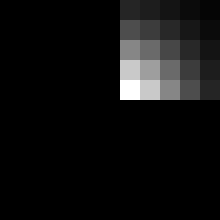
\includegraphics[width=0.23\textwidth]{./template_1_a.png}
% 			
\includegraphics[width=0.23\textwidth]{./template_1_b.png}
% 			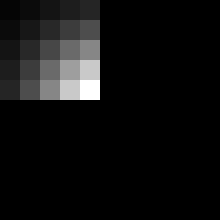
\includegraphics[width=0.23\textwidth]{./template_1_c.png}
% 			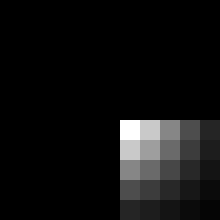
\includegraphics[width=0.23\textwidth]{./template_1_d.png}
% 			\caption{Corner prototype 1 (A, B, C, D)}
% 		\end{subfigure}
%
%     \vspace{0.5cm}
%
% 		\begin{subfigure}{0.48\textwidth}
% 			\centering
% 			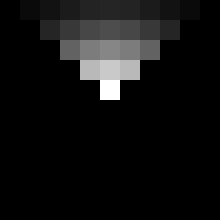
\includegraphics[width=0.23\textwidth]{./template_2_a.png}
% 			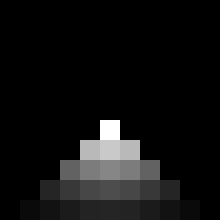
\includegraphics[width=0.23\textwidth]{./template_2_b.png}
% 			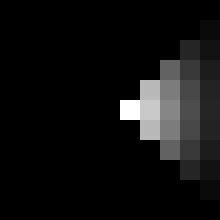
\includegraphics[width=0.23\textwidth]{./template_2_c.png}
% 			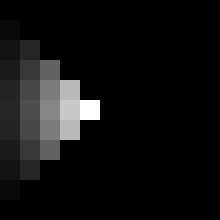
\includegraphics[width=0.23\textwidth]{./template_2_d.png}
% 			\caption{Corner prototype 2 (A, B, C, D)}
% 		\end{subfigure}
%
% 		\caption{Corner prototypes}
% 	\end{figure}
%
% \end{multicols}

\begin{figure}[h]
	\centering

	\begin{subfigure}{0.45\textwidth}
		\centering
		\begin{minipage}{\textwidth}
			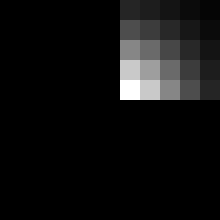
\includegraphics[width=0.24\textwidth]{./template_1_a.png}
			
\includegraphics[width=0.24\textwidth]{./template_1_b.png}
			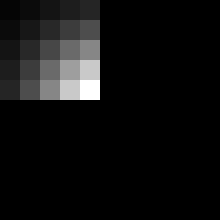
\includegraphics[width=0.24\textwidth]{./template_1_c.png}
			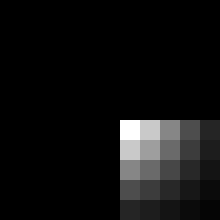
\includegraphics[width=0.24\textwidth]{./template_1_d.png}
		\end{minipage}
		\caption{Corner prototype 1 (A, B, C, D)}
	\end{subfigure}
	\hfill
	\begin{subfigure}{0.45\textwidth}
		\centering
		\begin{minipage}{\textwidth}
			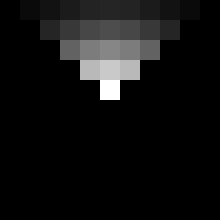
\includegraphics[width=0.24\textwidth]{./template_2_a.png}
			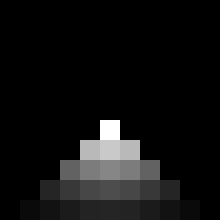
\includegraphics[width=0.24\textwidth]{./template_2_b.png}
			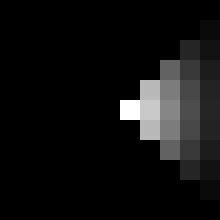
\includegraphics[width=0.24\textwidth]{./template_2_c.png}
			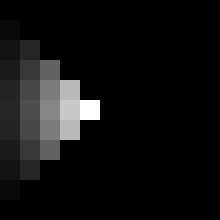
\includegraphics[width=0.24\textwidth]{./template_2_d.png}
		\end{minipage}
		\caption{Corner prototype 2 (A, B, C, D)}
	\end{subfigure}

	\caption{Corner prototypes \citep{geigerAutomaticCameraRange2012}}
	\label{fig:corner_prototypes}
\end{figure}

According to \cite{geigerAutomaticCameraRange2012}, the following approach proved to be
more robust to image clutter and blur than other common choices
\citep{harrisCombinedCornerEdge1988, shiGoodFeaturesTrack2000}.

To detect corners in a grayscale image $I$, the author used two $n \times n$ prototypes
for axis-aligned and $45^{\circ}$ rotated corners, respectively.
Each prototype
is constructed using four filter kernels $\{A, B, C, D\}$ (\cref{fig:corner_prototypes}). The corner likelihood
$c$ at each pixel is computed by:

\begin{equation}
	\begin{aligned}
		c     & =\max \left(s_1^1, s_2^1, s_1^2, s_2^2\right)                                             \\
		s_1^i & =\min \left(\min \left(f_A^i, f_B^i\right)-\mu, \mu-\min \left(f_C^i, f_D^i\right)\right) \\
		s_2^i & =\min \left(\mu-\min \left(f_A^i, f_B^i\right), \min \left(f_C^i, f_D^i\right)-\mu\right) \\
		\mu   & =0.25\left(f_A^i+f_B^i+f_C^i+f_D^i\right)
	\end{aligned}
\end{equation}

Then, the authors apply the conservative non-maximum suppression to the
response map, and additionally filter the corners by assuring that there are two
modes of the gradient directions.

\subsection{Sub-pixel Corner and Orientation Refinement}\label{sub:sub_pixel_corner_and_orientation_refinement}

Sub-pixel accurate corner locations and edge orientations are refined using the following optimizations:

For sub-pixel corner localization, the corner $\mathbf{c}$ in a 2D space
$\mathbb{R}^2$ is refined using the assumption that the gradient direction
\(\mathbf{g_{p}}\) at
each pixel  \(\mathbf{p}\) in the small neighbourhood around the corner is
orthogonal to \(\mathbf{p} - \mathbf{c}\).

\begin{equation}
	\mathbf{c}=\arg \min _{\mathbf{c}^{\prime}} \sum_{\mathbf{p} \in
	\mathcal{N}_{\mathbf{I}}\left(\mathbf{c}^{\prime}\right)}\left(\mathbf{g}_{\mathbf{p}}^T\left(\mathbf{p}-\mathbf{c}^{\prime}\right)\right)^2
\end{equation}

For the orientation refinement, authors minimize the distance from the
orientation vectors \(\mathbf{e_1}, \mathbf{e_2}\) to the gradient directions
\(\mathbf{g_p}\) in the neighbourhood of the corner.

\begin{equation}
	\mathbf{e}_i=\arg \min _{\mathbf{e}_i^{\prime}} \sum_{\mathbf{p} \in
		\mathcal{M}_i}\left(\mathbf{g}_{\mathbf{p}}^T \mathbf{e}_i^{\prime}\right)^2
	\quad \text { s.t. } \mathbf{e}_i^{\prime T} \mathbf{e}_i^{\prime}=1
\end{equation}.

The original paper then used a number of checks to further prune the detected
corners, and extending line by line the initial board, formed from the
random close points which made a square \todo{Make sure that's accurate, and
	reference. Also, the sentence is too compicated}.
We did not require that, since we already had the board, and we directly used
the response map to find the corners.

\missingfigure{Show the map of responses, and the detected corners}

To create a training dataset, we collected the true and false positives from the
corners we already had:

For each of the detected corners on all images, we collected the values of the
response function at the previously detected corners, and around them.
We didn't collect the values of all of the pixels, because then we would have
got too optimistic values for selecting the true positives\todo{Rephrase}.

\missingfigure{Show the distribution of the response function}

We trained a binary classifier, using the collected data, and then used it to
detect the true corners.



\chapter{Experiments}\label{cha:experiments}

\section{Simulator}\label{sec:simulator}

We created a simulator to generate distorted points as described in
\cref{sub:complete_projection_and_backprojection}. We used it to test the
solver and test the correctness of projection and back-projection points.
However, since the simulator used the same camera model as the solver, the
initial camera calibration was perfect.

\section{Metrics}\label{sec:metrics}

As noted by \cite{duisterhofTartanCalibIterativeWideAngle2022}, the evaluation
of the camera calibration is not straightforward. No ground truth exists for
feature detection or camera calibration.

Typically, the reprojection error is used as a metric for the camera
calibration, but it depends on multiple factors: type of the calibration
pattern, the camera model, and the types of the lens.

Also, by using more features, we can get better calibration, as we have more
constraints, but the reprojection error might be higher.

As currently the algorithm only supports processing a single checkerboard, we
cannot compare to \cite{duisterhofTartanCalibIterativeWideAngle2022}, which uses
AprilTags, nor to the \cite{lochmanBabelCalibUniversalApproach2021}, who
provides the detected corners for all of the boards.
\todo{Should I maybe tell less about it?}

Because of that, we instead artificially removed some of the points from the
detections, to ensure that we can recover them. We also created
artificially occluded points by overlaying a separate image, as it poses
problems for the feature detector.

Lastly, we evaluated the newly detected points on real-world datasets.

\section{Dataset}\label{sec:dataset}

For the project, we need highly distorted photos of calibration boards. It takes
a lot of work to generate such a dataset, as cameras which produce such images are
usually expensive. Therefore, it would be preferable to use an existing dataset.

For this project, we required a highly distorted dataset of chessboard images.
We collected several datasets, but the feature detector we used supports
detecting only the boards with the constant tile size, therefore we cannot use
AprilGrid nor CharuCO boards. The feature detector is the only limiting factor.

\textcite{lochmanBabelCalibUniversalApproach2021} collected a wide number of
datasets, typically used in the field for the benchmarking of the camera
calibration. They're provided in a Deltille \cite{DeltilleDetector2023} format,
and are well documented:

\textbf{Kalibr} \citep{mayeSelfsupervisedCalibrationRobotic2013} contains several established datasets that are commonly used for testing
the accuracy of camera calibration frameworks: Double Sphere
\cite{usenkoDoubleSphereCamera2018}, EuRoC \cite{burriEuRoCMicroAerial2016}, TUM
VI \cite{schubertTUMVIBenchmark2018}, and ENTANIYA 1
\cite{Calibration250degFisheye}.
The Kalibr calibration framework was used in the
original publications cited above, hence the name of the dataset.
As a calibration pattern, AprilGrid with 6x6 tags of 88 mm size was used.
In total, the datasets contain approximately 800 images.

\textbf{OCamCalib} \citep{scaramuzzaFlexibleTechniqueAccurate2006} is a dataset
of approximately 300 images.
As a calibration pattern, the checkerboard pattern of different sizes was used.

\textbf{UZH} \citep{AreWeReady} is a dataset of approximately 800 images
collected using the following cameras:
As a calibration pattern, AprilGrid with 4x5 tags of 75 mm size was used.
The dataset contains approximately 800 images.

\textbf{OV} \citep{lochmanBabelCalibUniversalApproach2021} is a dataset of
approximately 1400 images. It was collected using eight stereo cameras.
As a calibration pattern, the checkerboard pattern with 9x6 tags of 22 mm size
was used.

\textcite{duisterhofTartanCalibIterativeWideAngle2022} also provide their
dataset from the TartanCalib project. Currently, the dataset contains only
AprilGrid patterns, as the toolchain doesn't support a chessboard.

\begin{figure}[h]
	\centering
	\begin{subfigure}[b]{0.3\linewidth}
		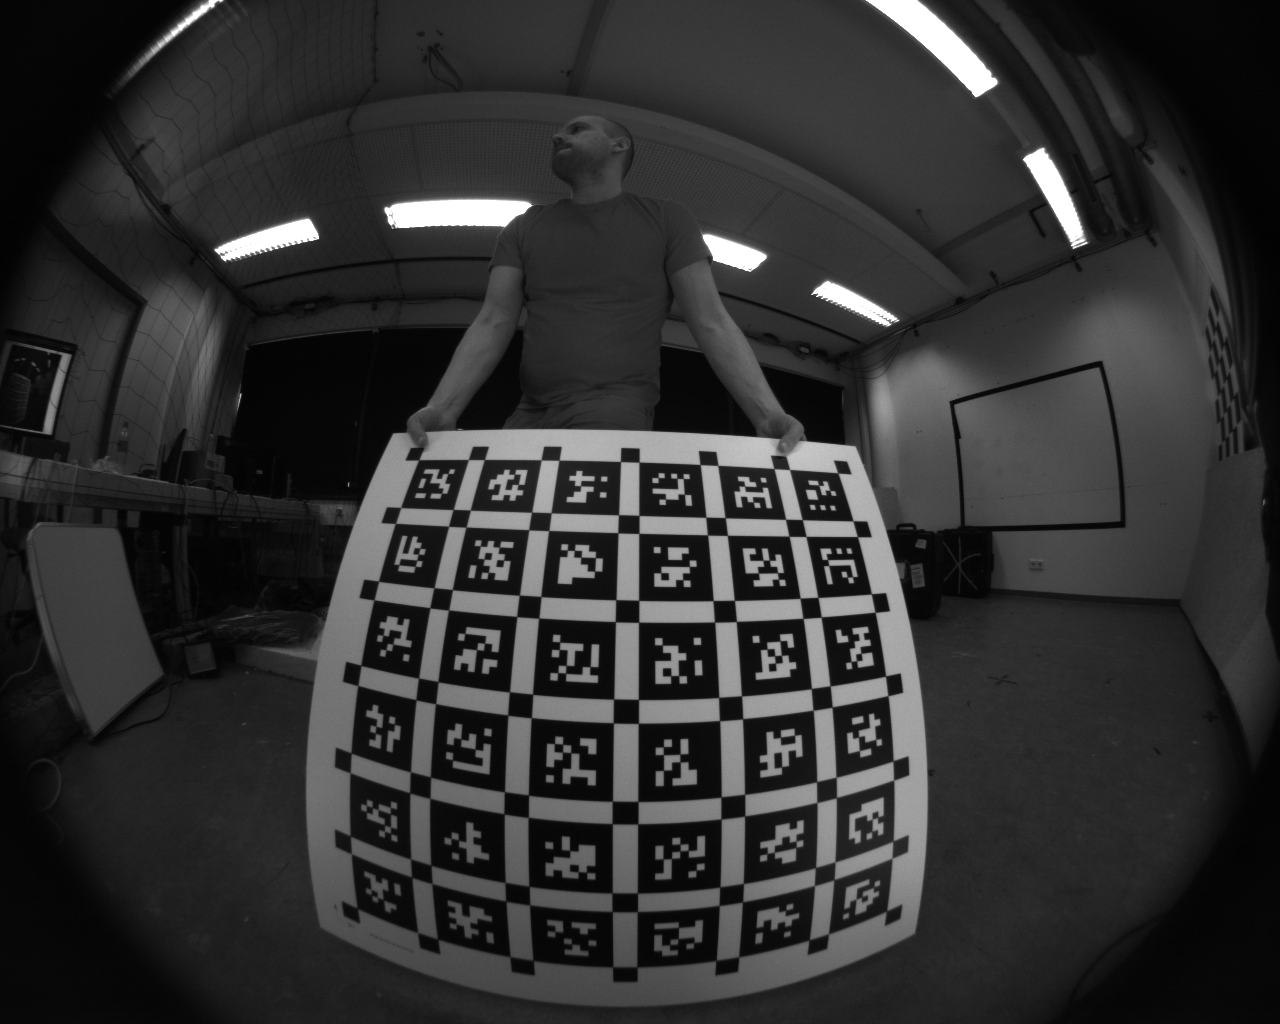
\includegraphics[width=\linewidth]{Kalibr.png}
		\caption{Kalibr}
	\end{subfigure}
	\hfill
	\begin{subfigure}[b]{0.3\linewidth}
		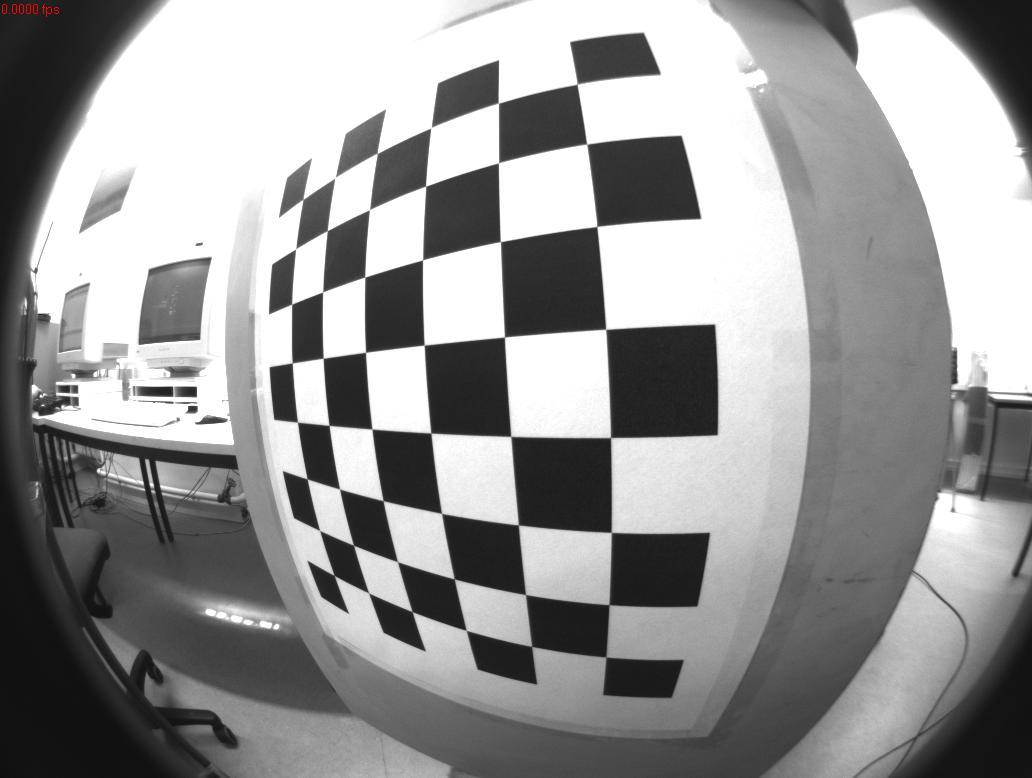
\includegraphics[width=\linewidth]{OCamCalib.png}
		\caption{\textbf{OCamCalib}}
	\end{subfigure}
	\hfill
	\begin{subfigure}[b]{0.3\linewidth}
		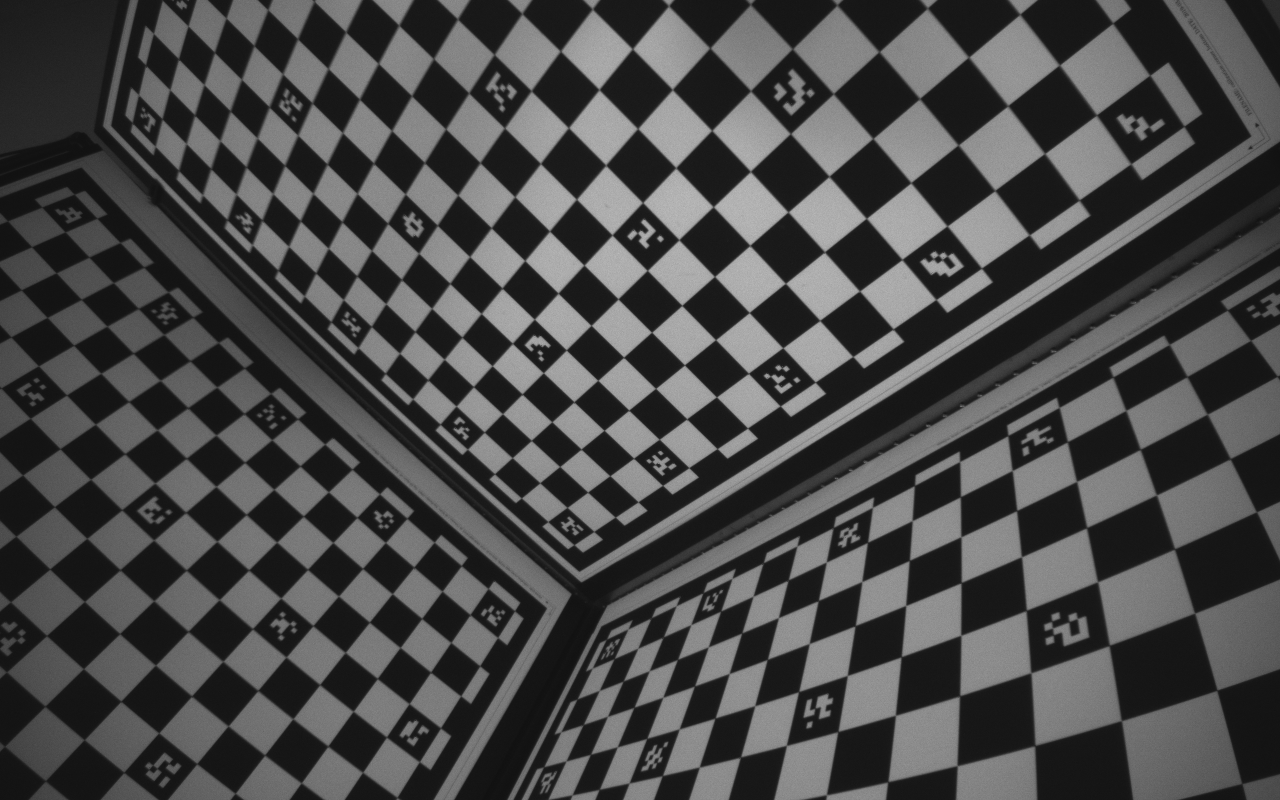
\includegraphics[width=\linewidth]{OV.png}
		\caption{\textbf{OV}}
	\end{subfigure}
	\begin{subfigure}[b]{0.3\linewidth}
		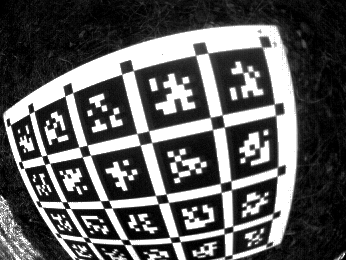
\includegraphics[width=\linewidth]{UZH.png}
		\caption{UZH}
	\end{subfigure}
	\begin{subfigure}[b]{0.3\linewidth}
		\includegraphics[width=\linewidth]{tartancalib.png}
		\caption{TartanCalib}
	\end{subfigure}
	\caption{Images from the datasets}
\end{figure}

\section{Camera calibration}\label{sec:camera_calibration}

\begin{minipage}{0.5\linewidth}
	To get accurate predictions for the possibly missing points, we need
	very accurate camera calibration. We used the reprojection error as a metric
	for the calibration quality.
	To calculate the reprojection error, we have to perform the
	rootfinding \cref{subsub:back_projection_using_the_division_model}. We assume
	that all of the points lay within the image, or they get out of the borders
	a little bit (we use the constant \(1.1\) of the maximum radius). If the
	camera calibration is poor, the root-finding might fail. On the initial
	calibration the number of the failed root-findings was much higher.
\end{minipage}
\hfill
\begin{minipage}{0.4\linewidth}
	\resizebox{\linewidth}{!}{
		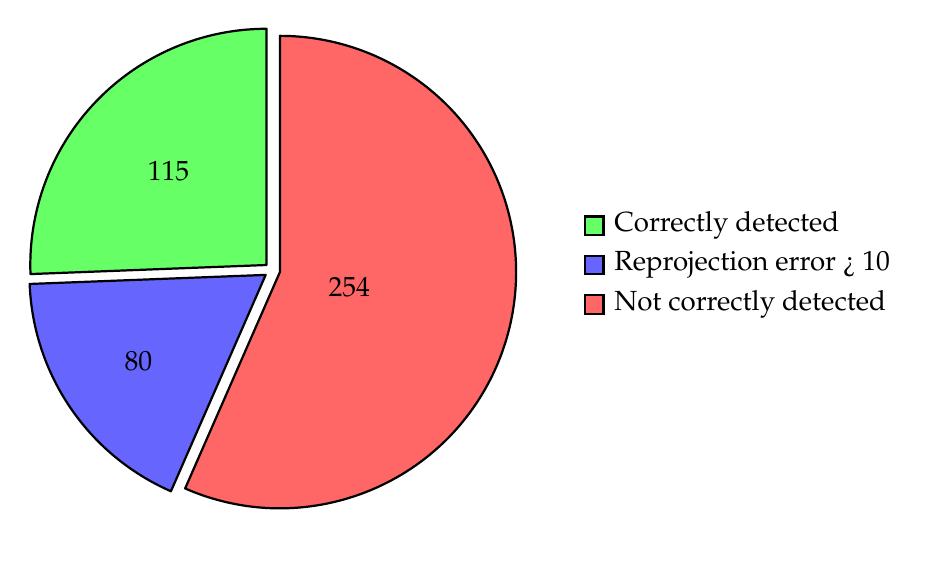
\begin{tikzpicture}
			\pie[rotate=90, explode=0.1, sum=auto, color={green!60, blue!60, red!60}, text=legend]{
				115/Correctly detected,
				80/Reprojection error > 10,
				254/Not correctly detected
			}
		\end{tikzpicture}
	}
	\captionsetup{width=.9\linewidth}
	\captionof{figure}{Initial calibration}
	\resizebox{\linewidth}{!}{
		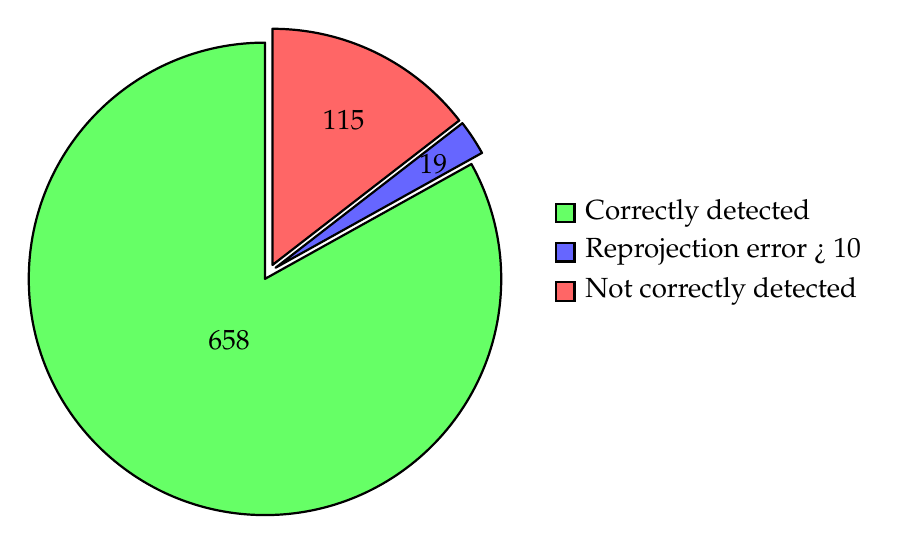
\begin{tikzpicture}
			\pie[rotate=90, explode=0.1, sum=auto, color={green!60, blue!60, red!60}, text=legend]{
				658/Correctly detected,
				19/Reprojection error > 10,
				115/Not correctly detected
			}
		\end{tikzpicture}
	}
	\captionsetup{width=.9\linewidth}
	\captionof{figure}{Final calibration}
\end{minipage}

\begin{figure}[h]
	\begin{tikzpicture}
		\begin{axis}[
				ybar interval,
				ymin=0,
				ylabel={Frequency},
				xlabel={Value},
				height=0.3\linewidth,
				width=\linewidth,
				ticklabel style = {font=\tiny},
				% title={Initial calibration}
			]
			\addplot+ [hist={data min=0,data max=10,bins=20}] table [y index=0]
				% \addplot+ [hist={bins=30}] table [y index=0]
				{data/reprojection_error_init.txt};
		\end{axis}
	\end{tikzpicture}
	\caption{Initial calibration's reprojection error histogram}
\end{figure}
\begin{figure}[h]
	\begin{tikzpicture}
		\begin{axis}[
				ybar interval,
				ymin=0,
				ylabel={Frequency},
				xlabel={Value},
				height=0.3\linewidth,
				width=\linewidth,
				ticklabel style = {font=\tiny},
				% title={Reprojection error}
			]
			\addplot+ [hist={data min=0,data max=10,bins=20}] table [y index=0]
				% \addplot+ [hist={bins=30}] table [y index=0]
				{data/reprojection_error_final.txt};
		\end{axis}
	\end{tikzpicture}
	\caption{Final calibration's reprojection error histogram}
\end{figure}

\section{Additional features detection}\label{sec:additional_features_detection}

As discussed in \cref{sec:additional_features_detection}, we filled the gaps in
the originally detected board points, and then padded it for 1 additional
element.

\begin{figure}[h]
	\centering
	\begin{minipage}{0.55\linewidth}
		\begin{subfigure}[b]{\linewidth}
			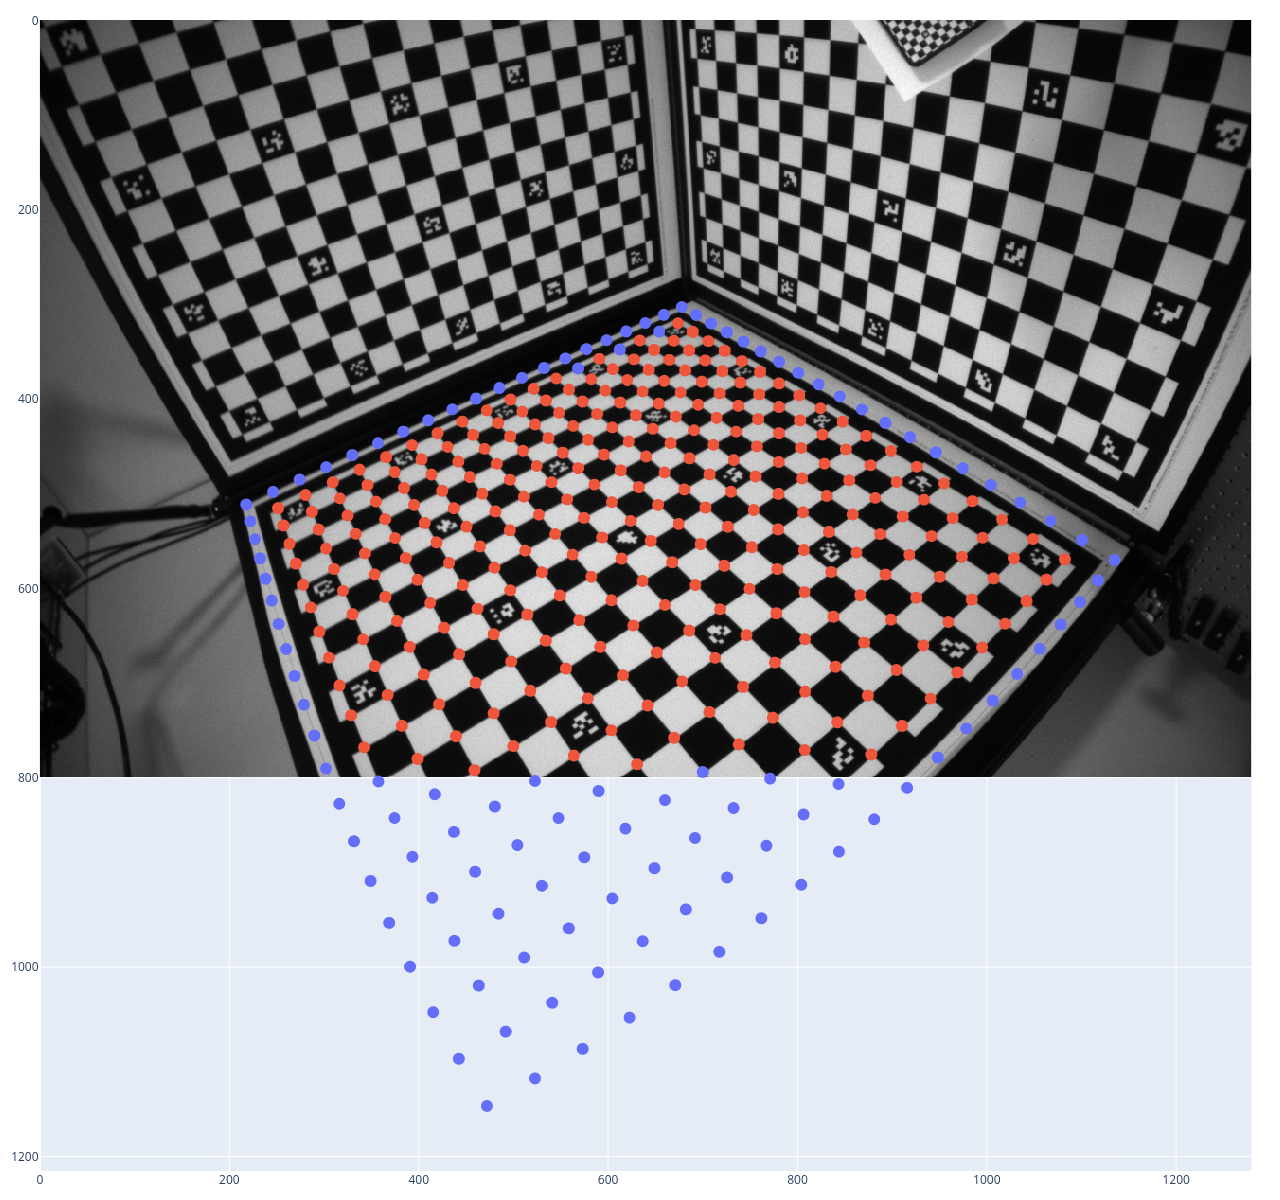
\includegraphics[width=\linewidth]{extended_board_img.png}
			\label{fig:extended_board_img}
			\caption{Extended board, new points are marked as blue}
		\end{subfigure}
	\end{minipage}
	\begin{minipage}{0.35\linewidth}
		\resizebox{\linewidth}{!}{
			\begin{tikzpicture}
				\begin{axis}[
						xlabel={$x$},
						ylabel={$y$},
						grid=major,
						title={Original board},
					]
					\addplot[
						only marks,
					] table {data/original_board.txt};
				\end{axis}
			\end{tikzpicture}
		}
		\vfill
		\resizebox{\linewidth}{!}{
			\centering
			\begin{tikzpicture}
				\begin{axis}[
						xlabel={$x$},
						ylabel={$y$},
						grid=major,
						title={Extended board},
					]
					\addplot[
						only marks,
					] table {data/extended_board.txt};
				\end{axis}
			\end{tikzpicture}
		}
	\end{minipage}
	\caption{Board extension}
\end{figure}

\section{Classification}\label{sec:classification}

\begin{minipage}[t]{0.3\linewidth}
	We compared both responses, as discussed in \cref{sec:classifier}.
	The Hessian proved to be more robust. The approach, proposed by
	\cite{geigerAutomaticCameraRange2012} gave too many false positives,
	especially for the edges.
\end{minipage}
\hfill
\begin{minipage}[t]{0.6\linewidth}
	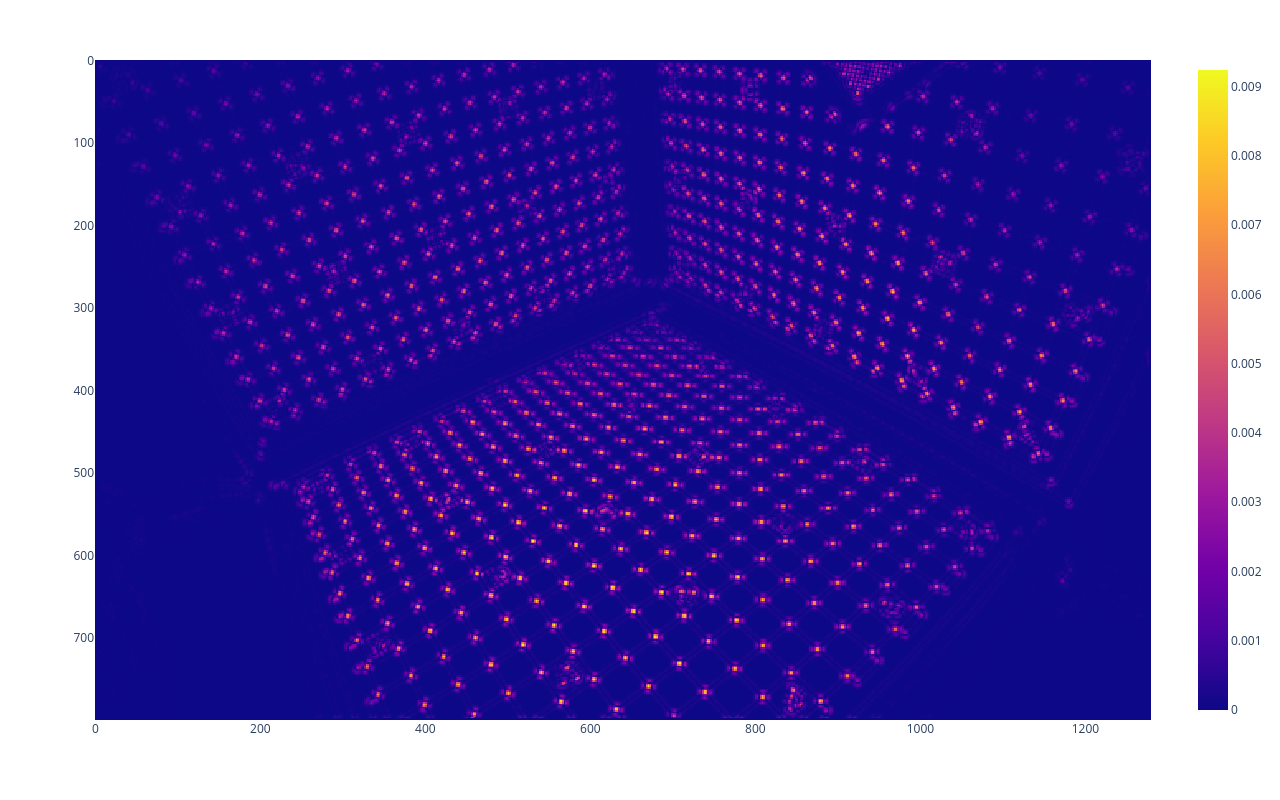
\includegraphics[width=\linewidth]{response_hessian.png}
	\captionof{figure}{Hessian response}
	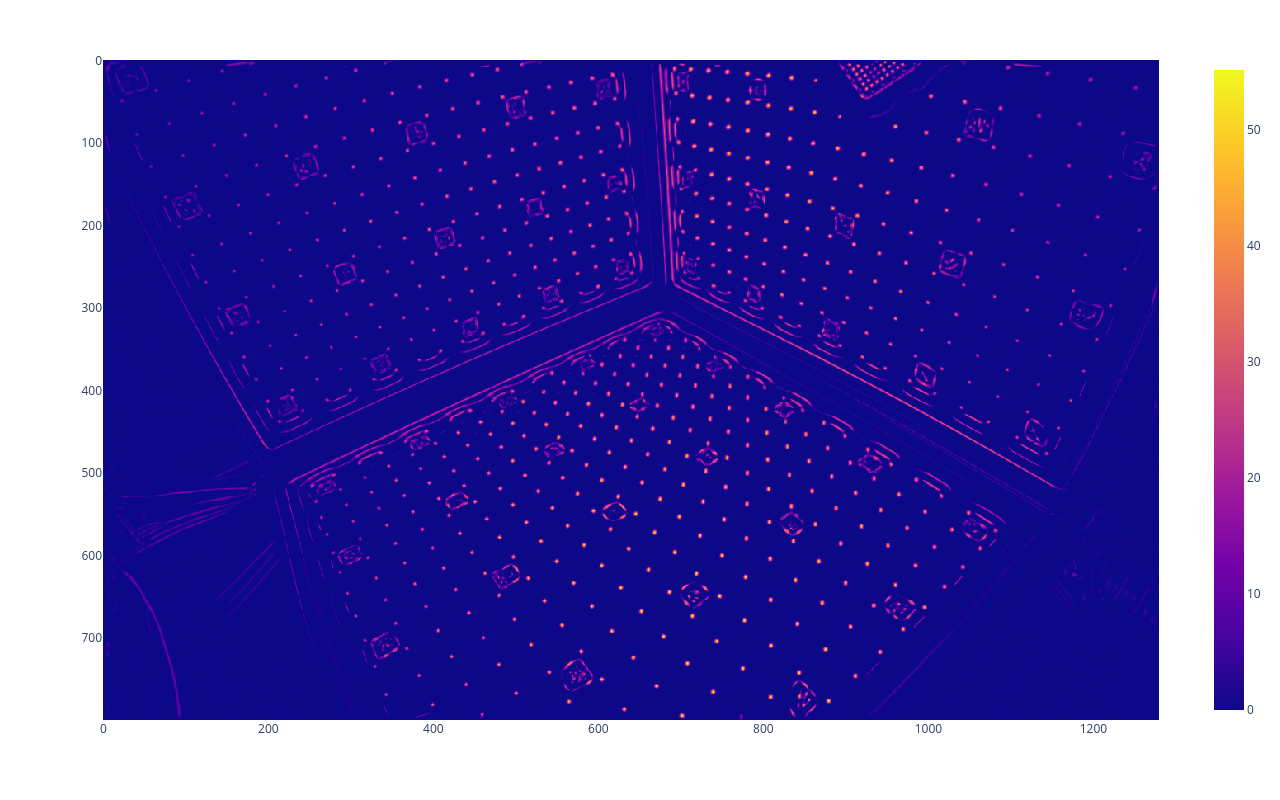
\includegraphics[width=\linewidth]{response_other.png}
	\captionof{figure}{Response used by \cite{geigerAutomaticCameraRange2012}}
	% \end{figure}
\end{minipage}

\begin{figure}
	\centering
	\begin{subfigure}[t]{0.45\linewidth}
		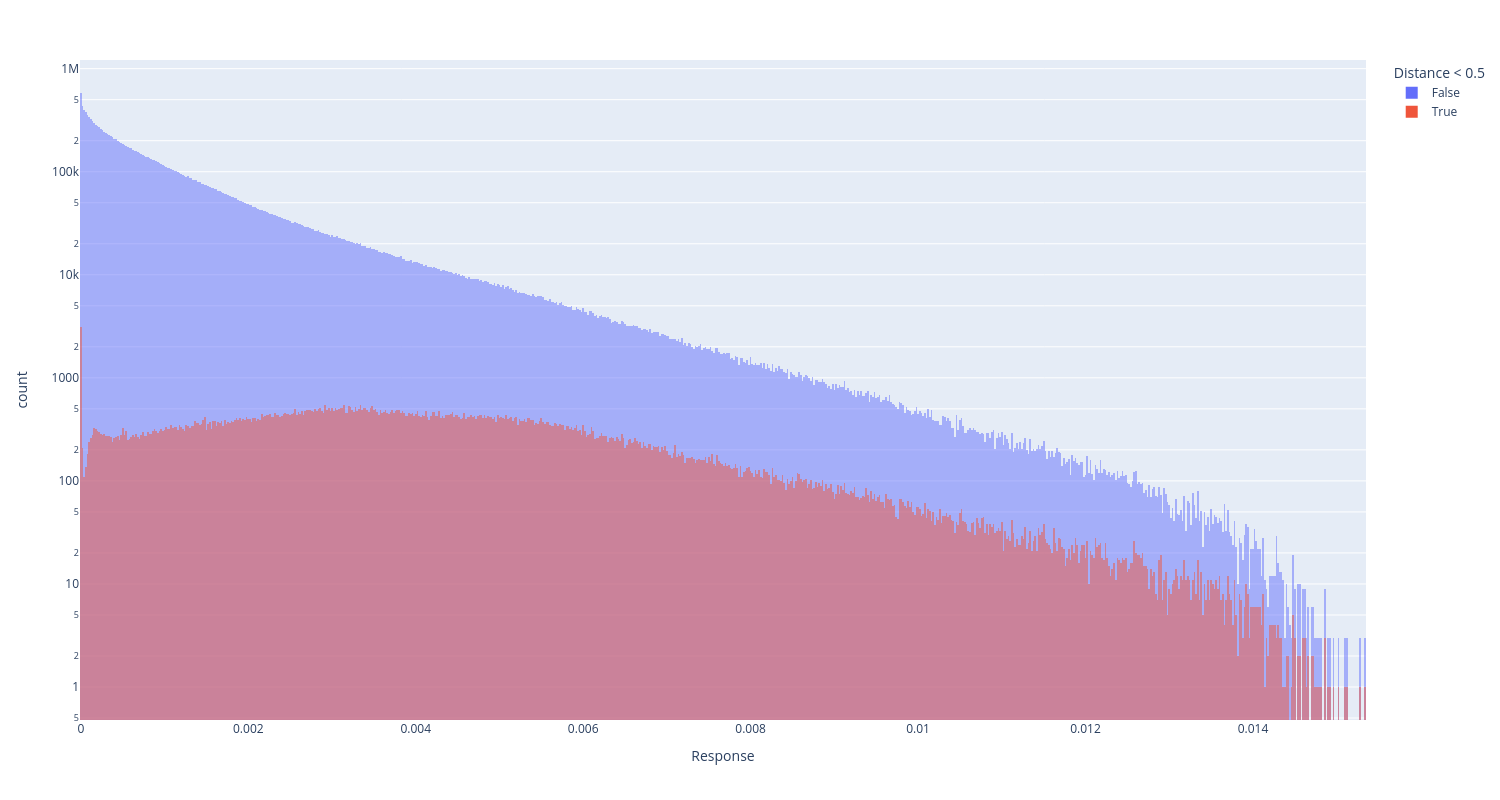
\includegraphics[width=\linewidth]{hist_response_hessian.png}
		\caption{Histogram of Hessian response}
	\end{subfigure}
	\begin{subfigure}[t]{0.45\linewidth}
		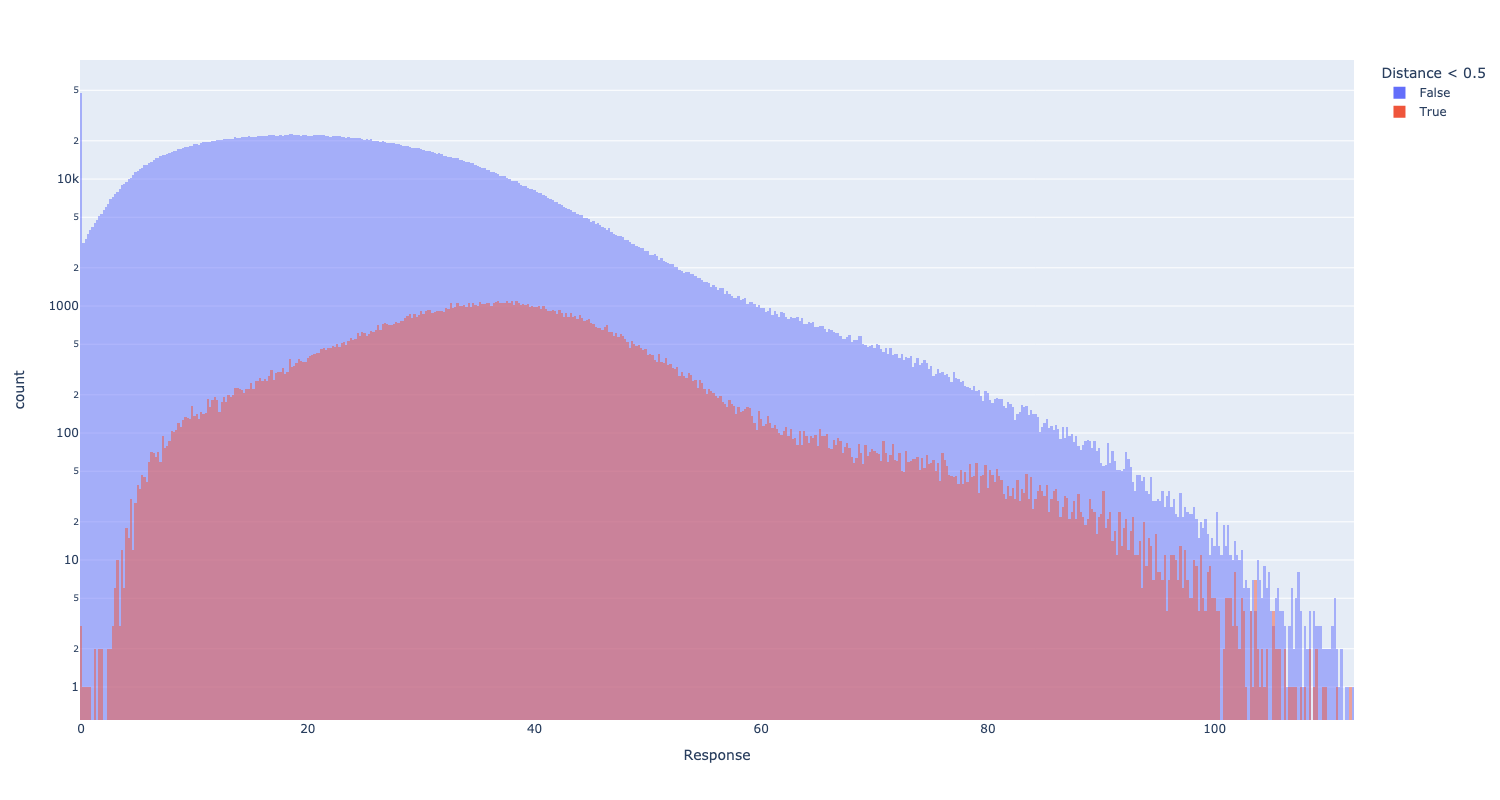
\includegraphics[width=\linewidth]{hist_response_other.png}
		\caption{Histogram of response used by \cite{geigerAutomaticCameraRange2012}}
	\end{subfigure}
	\caption{Distributions of the responses for the image on the
		\cref{fig:extended_board_img}. Note the log y-scale! Most of the points have
		the response 0.}
\end{figure}

\section{Evaluation}\label{sec:evaluation}

\subsection{Recovery of artificially removed points}\label{sub:recovery_of_artificially_removed_points}

We removed 20\% of the points from the original board, and then tried to recover
them.

\begin{figure}[h]
	\centering
	\begin{subfigure}[h]{0.45\linewidth}
		\begin{tikzpicture}
			\begin{axis}[
					ybar interval,
					ymin=0,
					ylabel={Frequency},
					xlabel={Value},
					height=0.5\linewidth,
					width=\linewidth,
					ticklabel style = {font=\tiny},
					title={Histogram of the points before refinement}
				]
				\addplot+ [hist={data min=0,data max=600,bins=10}] table [y index=0]
					% \addplot+ [hist={bins=30}] table [y index=0]
					{data/pruned_number_of_features.txt};
			\end{axis}
		\end{tikzpicture}
	\end{subfigure}
	\hfill
	\begin{subfigure}[h]{0.45\linewidth}
		% \centering
		\begin{tikzpicture}
			\begin{axis}[
					ybar interval,
					ymin=0,
					ylabel={Frequency},
					xlabel={Value},
					height=0.5\linewidth,
					width=\linewidth,
					ticklabel style = {font=\tiny},
					title={Histogram of the points after refinement}
				]
				\addplot+ [hist={data min=0,data max=600,bins=10}] table [y index=0]
					% \addplot+ [hist={bins=30}] table [y index=0]
					{data/recovered_pruned_number_of_features.txt};
			\end{axis}
		\end{tikzpicture}
	\end{subfigure}
	\begin{subfigure}[h]{\linewidth}
		\centering
		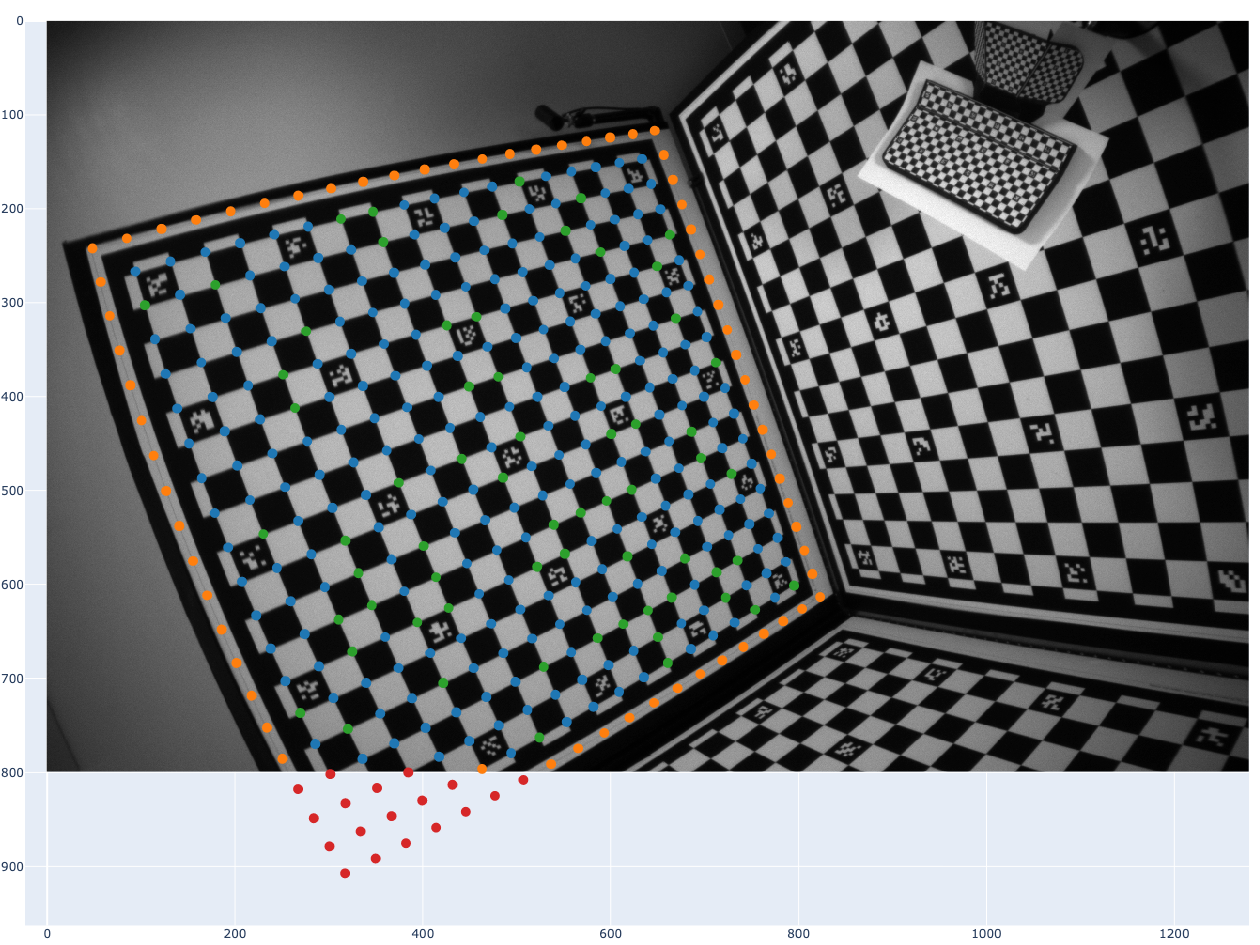
\includegraphics[width=0.7\linewidth]{refined_pruned_corners.png}
		\caption{Recovered pruned points
			(\textcolor[HTML]{1f77b4}{unchanged}
			\textcolor[HTML]{ff7f0e}{filtered out}
			\textcolor[HTML]{2ca02c}{new corner}
			\textcolor[HTML]{d62728}{out of image})}
	\end{subfigure}
	\hfill
	\caption{Feature refinement on the board with 80\% of the points}
\end{figure}

\newpage
\subsection{Performance under occlusion}\label{sub:performance_under_occlusion}

Occlusions pose additional complications for the feature detection. We added an
image on top of the board, and tried to recover additional points. Often the
initial feature detector failed to detect points near the occlusion.

\begin{figure}[h]
	\centering
	\begin{subfigure}[h]{0.45\linewidth}
		\begin{tikzpicture}
			\begin{axis}[
					ybar interval,
					ymin=0,
					ylabel={Frequency},
					xlabel={Value},
					height=0.5\linewidth,
					width=\linewidth,
					ticklabel style = {font=\tiny},
					title={Histogram of the points before the refinement}
				]
				\addplot+ [hist={data min=0,data max=500,bins=20}] table [y index=0]
					% \addplot+ [hist={bins=30}] table [y index=0]
					{data/occluded_number_of_features.txt};
			\end{axis}
		\end{tikzpicture}
		\caption{}
	\end{subfigure}
	\hfill
	\begin{subfigure}[h]{0.45\linewidth}
		% \centering
		\begin{tikzpicture}
			\begin{axis}[
					ybar interval,
					ymin=0,
					ylabel={Frequency},
					xlabel={Value},
					height=0.5\linewidth,
					width=\linewidth,
					ticklabel style = {font=\tiny},
					title={Histogram of the points after the refinement}
				]
				\addplot+ [hist={data min=0,data max=500,bins=20}] table [y index=0]
					% \addplot+ [hist={bins=30}] table [y index=0]
					{data/recovered_occluded_number_of_features.txt};
			\end{axis}
		\end{tikzpicture}
	\end{subfigure}
	\begin{subfigure}[h]{\linewidth}
		\centering
		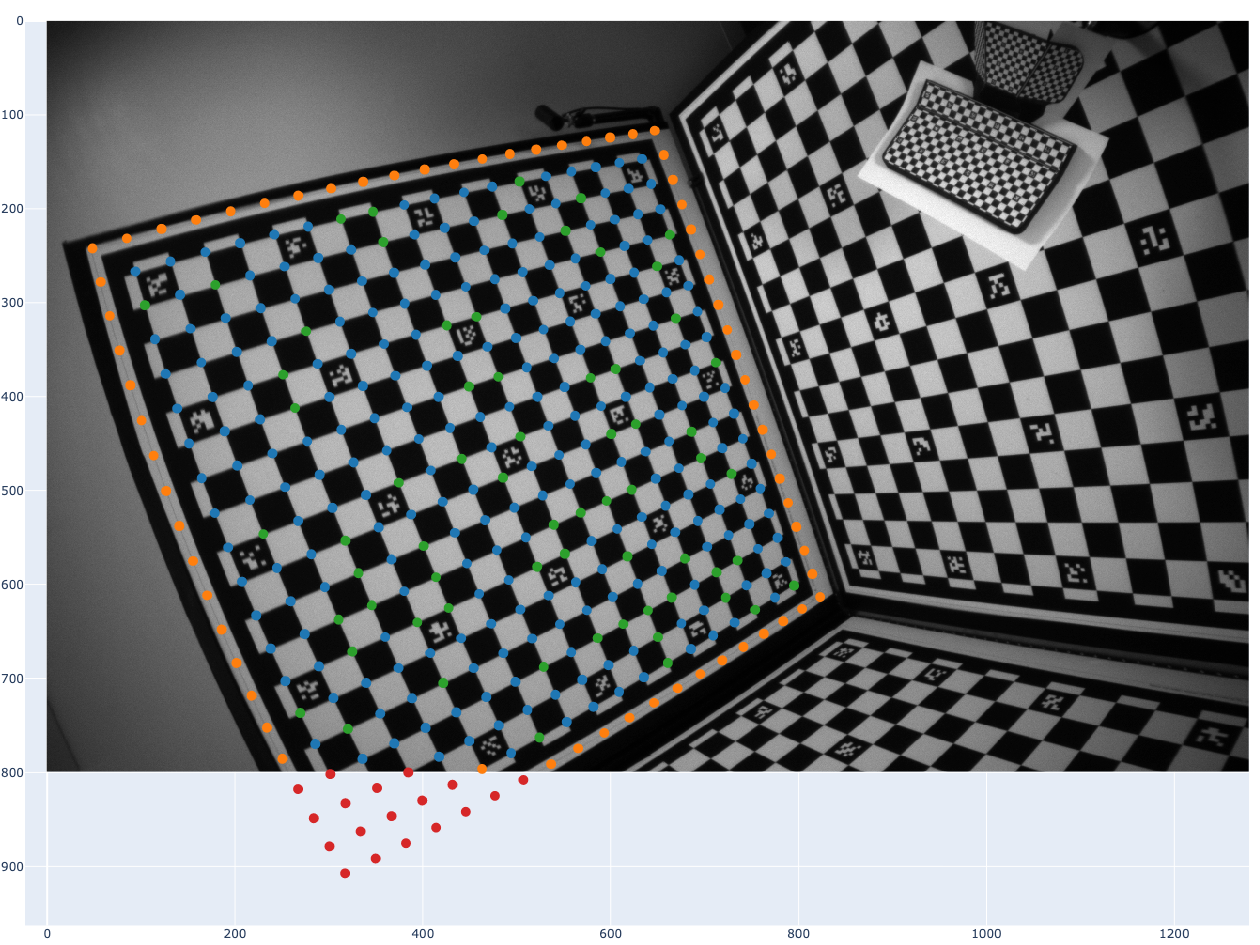
\includegraphics[width=0.7\linewidth]{refined_pruned_corners.png}
		\caption{Recovered pruned points
			(\textcolor[HTML]{1f77b4}{unchanged}
			\textcolor[HTML]{ff7f0e}{filtered out}
			\textcolor[HTML]{2ca02c}{new corner}
			\textcolor[HTML]{d62728}{out of image})}
	\end{subfigure}
	\hfill
	\caption{Feature refinement on the board with partial board occlusion}
\end{figure}

\newpage
\subsection{Recovery of previously undetected points}\label{sub:recovery_of_previously_undetected_points}

\begin{minipage}[t]{0.3\linewidth}
	Lastly, we recovered the points that were not detected by the initial feature
	detector.
	From a visual inspection, most of the points were recovered correctly
	\cref{fig:recovered_good_points}.
	On the top image, for example, there are green points close to the edge.
	Those corners weren't detected initially due to high distortion. On the bottom
	image, the algorithm found another row of the corners, which weren't detected previously.
\end{minipage}
\hfill
\begin{minipage}[t]{0.6\linewidth}
	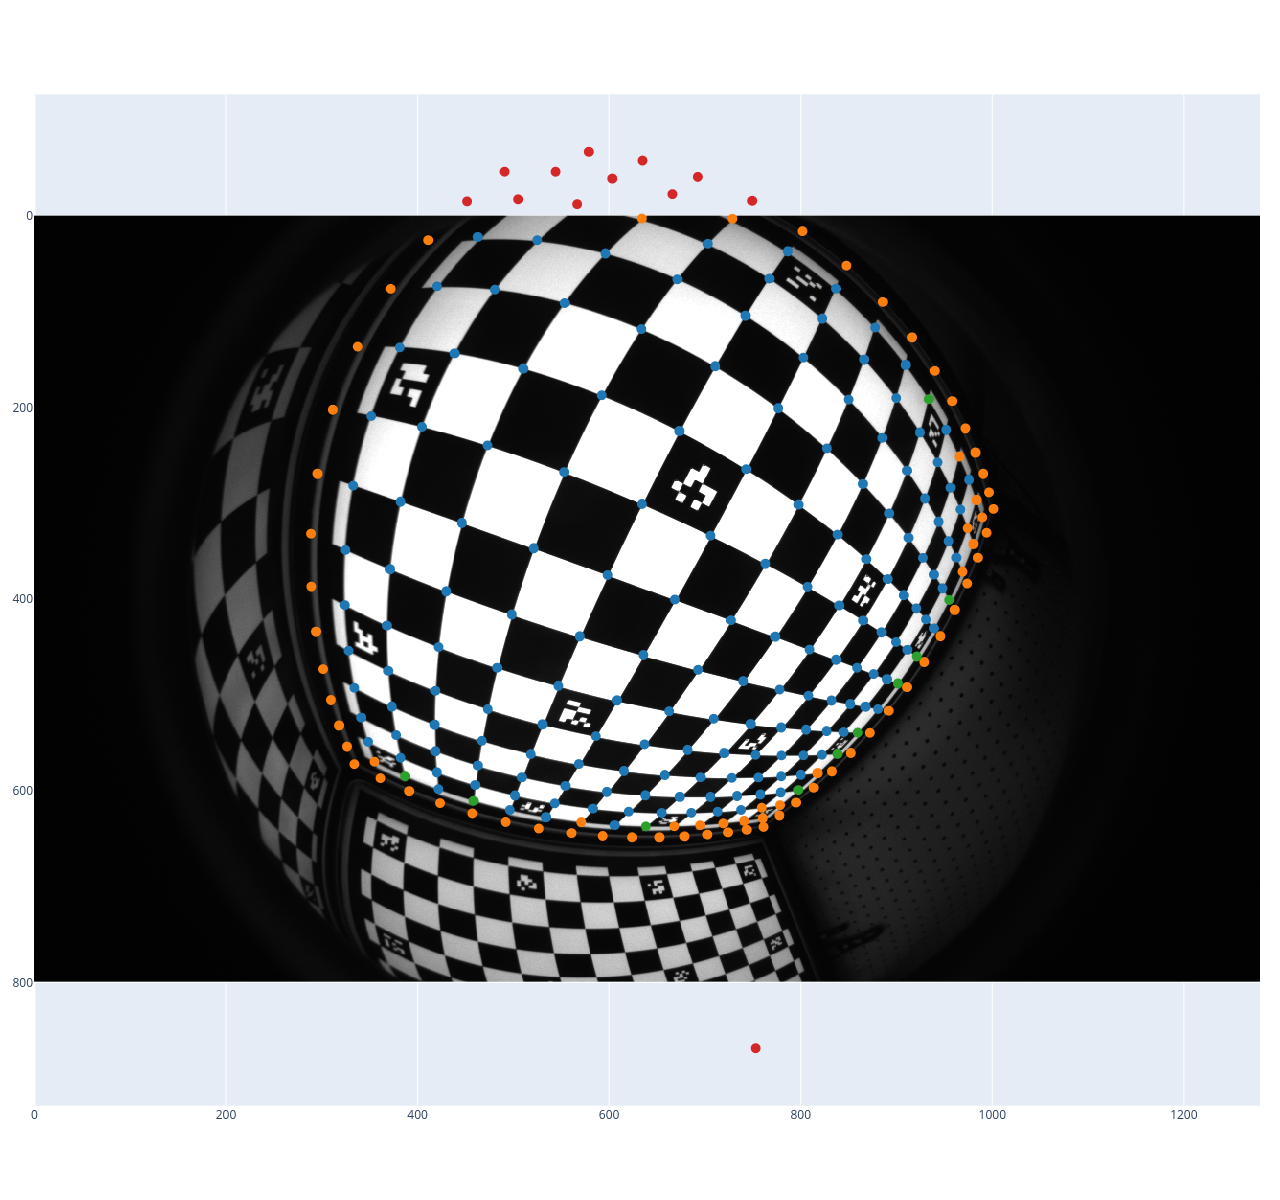
\includegraphics[width=\linewidth]{refined_corners1.png}
	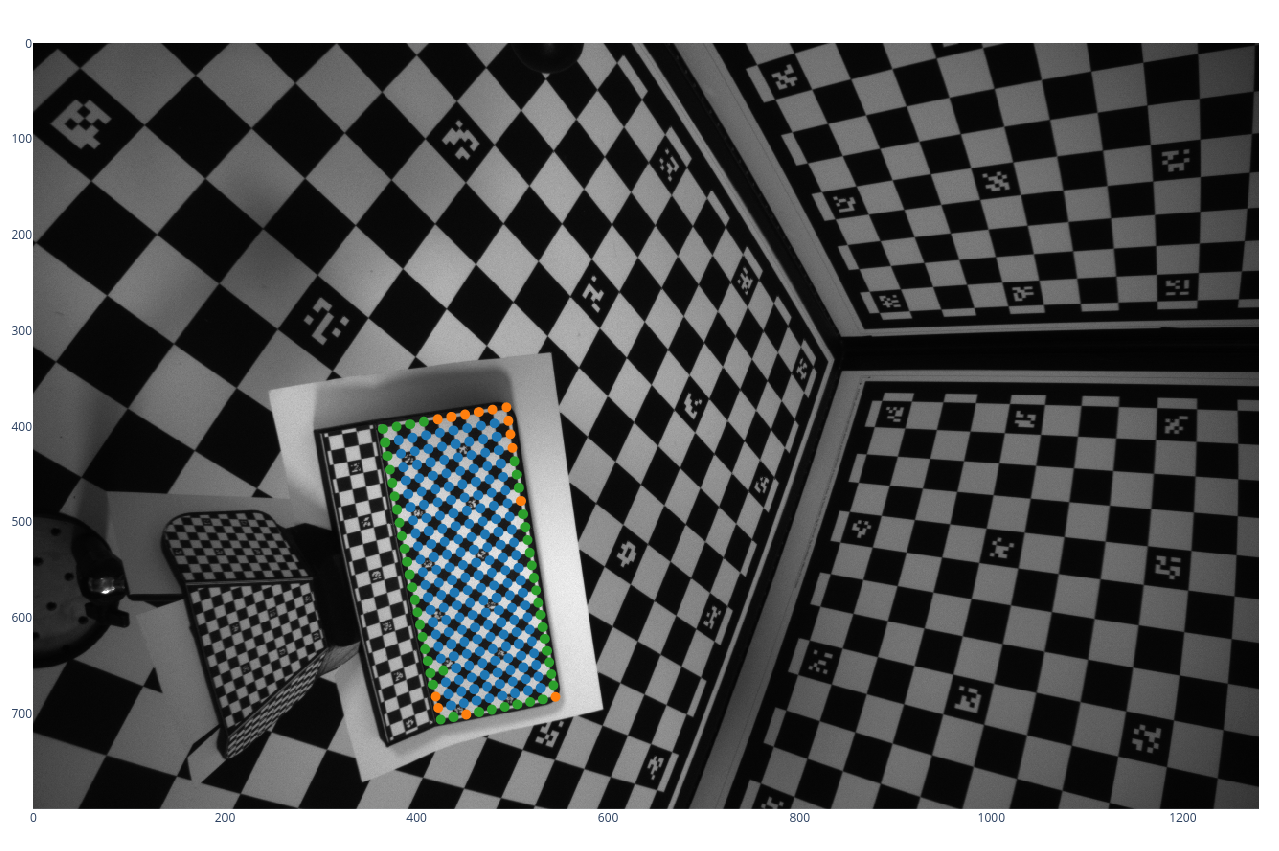
\includegraphics[width=\linewidth]{refined_corners2.png}

	\captionof{figure}{Recovered points
		(\textcolor[HTML]{1f77b4}{unchanged}
		\textcolor[HTML]{ff7f0e}{filtered out}
		\textcolor[HTML]{2ca02c}{new corner}
		\textcolor[HTML]{d62728}{out of image})}
	\label{fig:recovered_good_points}
\end{minipage}

\begin{minipage}[t]{0.3\linewidth}
	However,
	because of the occlusions, or similar to the board patterns in the background,
	there were false positives \cref{fig:recovered_bad_points}. Many images didn't
	have undetected corners, hence it's hard to make a general statement about the
	performance of the feature detector solely based on this experiment
	\cref{fig:recovered_points_histogram}.
\end{minipage}
\hfill
\begin{minipage}[t]{0.6\linewidth}
	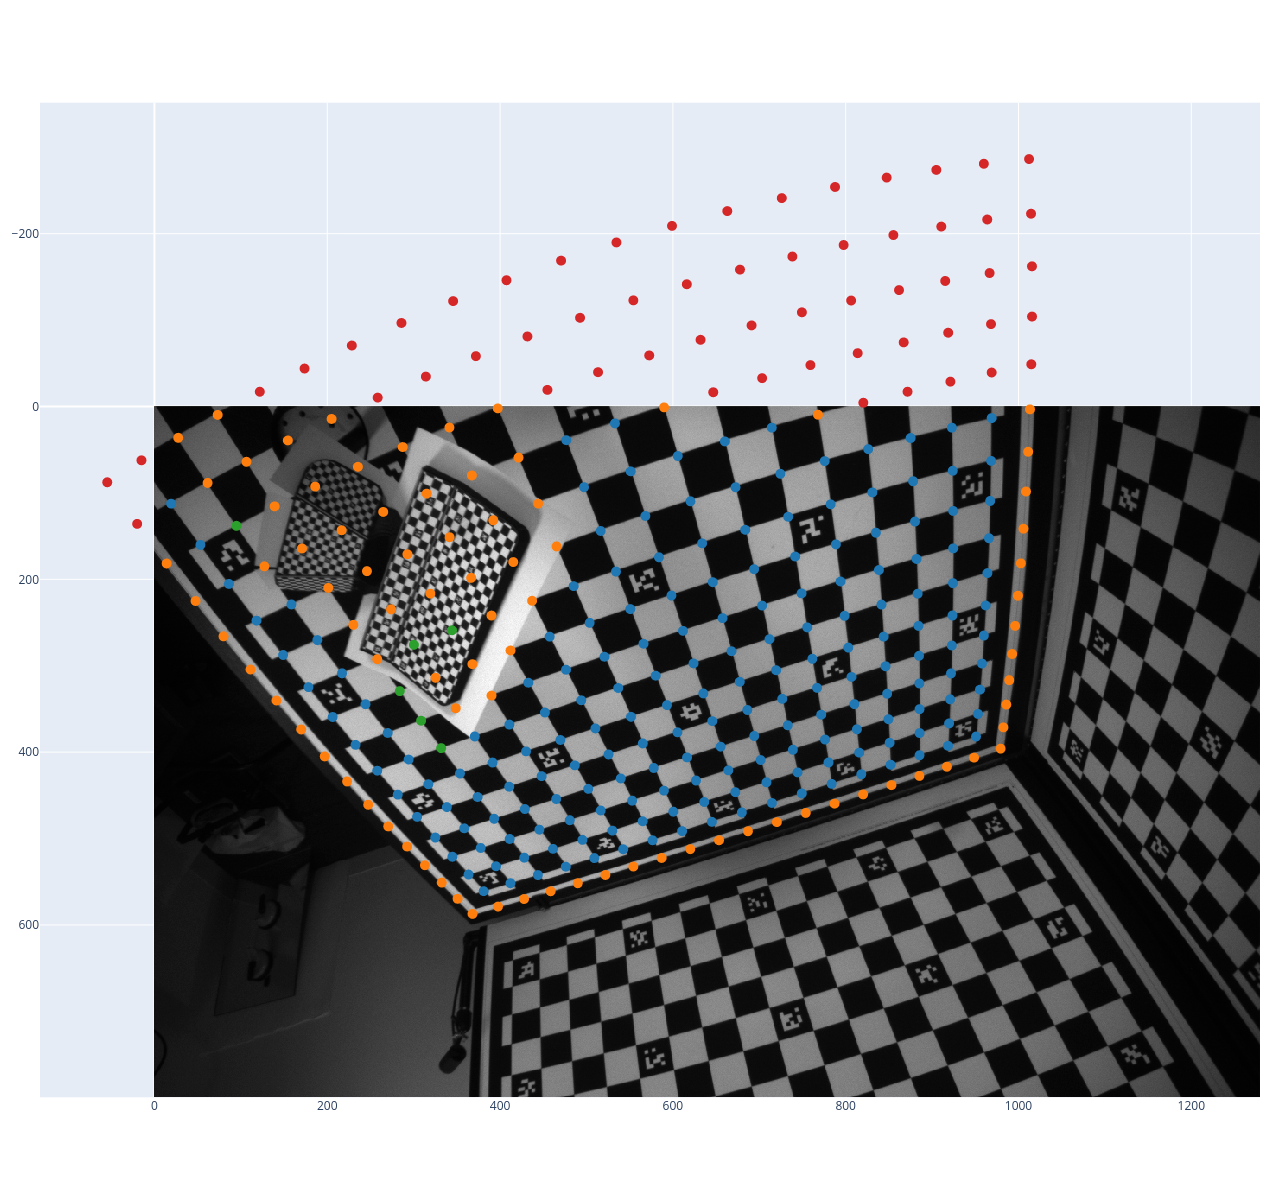
\includegraphics[width=\linewidth]{refined_corners_bad.png}
	\captionof{figure}{Occlusion on the board with distinct features}
	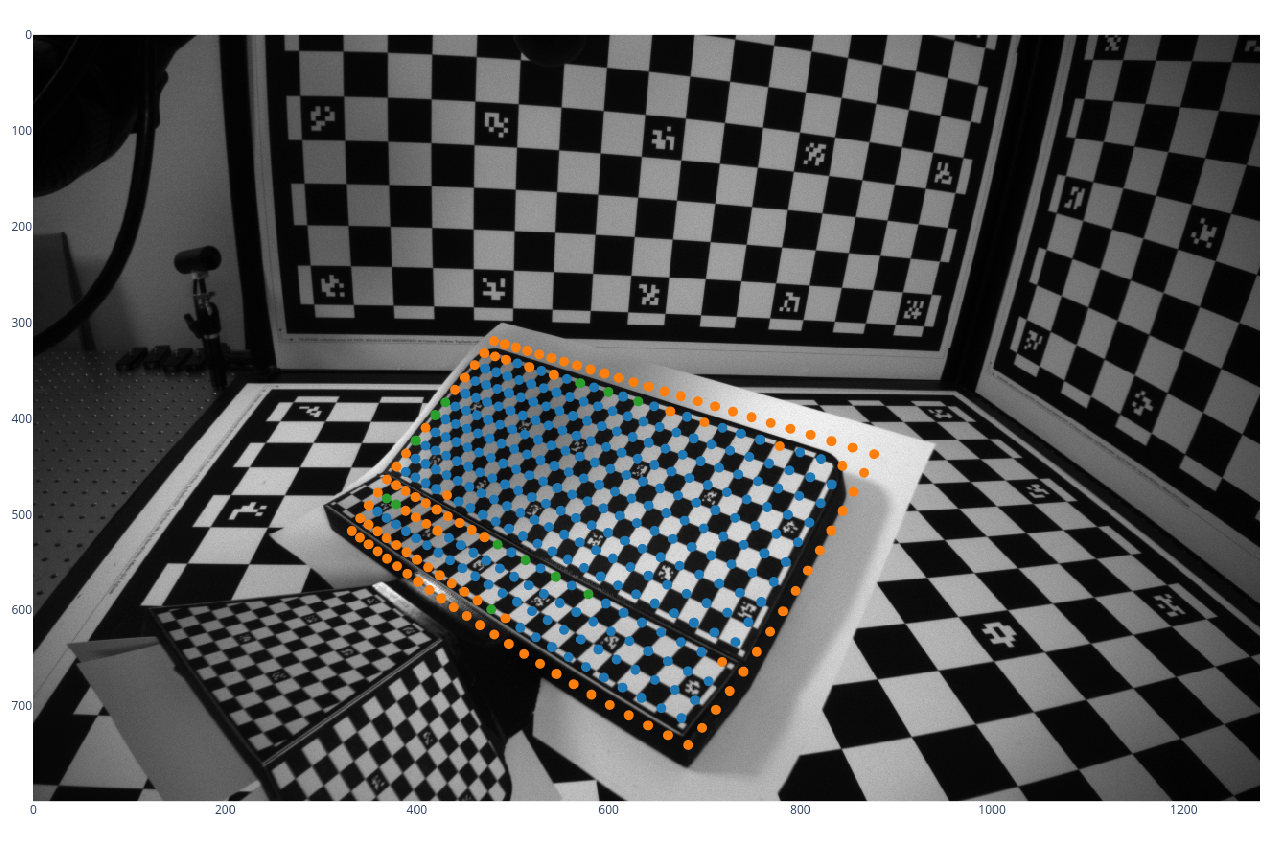
\includegraphics[width=\linewidth]{refined_corners_bad_bad.png}
	\captionof{figure}{Similar pattern to the board in the background}
	\label{fig:recovered_bad_points}
\end{minipage}

\begin{figure}[h]
	\begin{tikzpicture}
		\begin{axis}			[
				ymode=log,
				ybar interval,
				ymin=0,
				ylabel={Frequency},
				xlabel={Value},
				height=0.3\linewidth,
				width=\linewidth,
				ticklabel style = {font=\tiny},
				% title={Initial calibration}
			]
			\addplot+ [hist={data min=0,data max=100,bins=20}] table [y index=0]
				% \addplot+ [hist={bins=30}] table [y index=0]
				{data/number_of_refined_points.txt};
		\end{axis}
	\end{tikzpicture}
	\caption{Histogram of the newly recovered features}
	\label{fig:recovered_points_histogram}
\end{figure}



\chapter{Conclusions}\label{cha:conclusions}




%----------------------------------------------------------------------------------------
%	THESIS CONTENT - APPENDICES
%----------------------------------------------------------------------------------------

\appendix % Cue to tell LaTeX that the following "chapters" are Appendices

% Include the appendices of the thesis as separate files from the Appendices folder
% Uncomment the lines as you write the Appendices

% 
\chapter{Code}

\section{Pseudocode}

Something on the topic



\endinput
%\include{Appendices/AppendixB}
%\include{Appendices/AppendixC}

%----------------------------------------------------------------------------------------
%	BIBLIOGRAPHY
%----------------------------------------------------------------------------------------

\printbibliography[heading=bibintoc]

%----------------------------------------------------------------------------------------

\end{document}


